\documentclass{report}

%\usepackage{times}
\usepackage[pdftex,
  colorlinks=true,
  pdfstartview=FitV,
  linkcolor=blue,
  citecolor=blue,
  urlcolor=blue]{hyperref}
\usepackage{geometry}
\geometry{a4paper}
\usepackage{amssymb}
%\usepackage{epstopdf}
\usepackage{xspace}
\usepackage{indentfirst}

\usepackage[francais]{babel}
\usepackage[latin1]{inputenc}
\usepackage[dvips]{graphicx}
\usepackage{array}
\usepackage{multirow}
\usepackage{fancyheadings}
\usepackage[Lenny]{fncychap}
\pagestyle{fancy}
\newcommand{\sauteligne}{\vspace{0.5cm}}

\newcommand{\visidia}{ViSiDiA\xspace}
\newcommand{\berlios}{BerliOs.de\xspace}
\newcommand{\labri}{LaBRI\xspace}

\author{}
\date{}

\title{
  \begin{flushright}
    \begin{Huge}
      \begin{textbf}
        Projet \visidia\\
      \end{textbf}
    \end{Huge}
    \rule{\textwidth}{2mm}\\
    \large\rm{Rapport}\\
    \vspace{2cm}
    \begin{textbf}\\
      \underline{Auteurs} :\\
      \vspace{0.5cm}
      \sc Nada Ayad\\
      Damien Cassou\\
      Xavier Durand\\
      Jean-Baptiste Gautron\\
      Hicham Ghriss\\
      Mathieu Hopmann\\
      Julie Quagliozzi\\
      \vspace{5mm}
    \end{textbf}
    \rm \today
  \end{flushright}
}

\begin{document}
% \sloppy %�vite que les paragraphes ne d�passent. 
\maketitle
\tableofcontents

\chapter{R�sum�}

\paragraph{Pr�sentation g�n�rale}

La g�n�ralisation  des r�seaux h�t�rog�nes et de  grandes tailles dans
de   multiples   domaines  implique   des   �tudes  cons�quentes   sur
l'algorithmique    distribu�e.    Le    d�veloppement   d'applications
distribu�es est rendu difficile d�  � des probl�mes de concurrence aux
ressources et � la communication inter processus. C'est la raison pour
laquelle  les chercheurs ont  commenc� �  d�velopper des  logiciels de
simulation.    Ces   logiciels   permettent  de   suivre   l'�volution
d'algorithmes distribu�s graphiquement et en temps r�el dans le but de
comprendre leur fonctionnement, d'en  concevoir de nouveaux mais aussi
dans le but de trouver des propri�t�s et des invariants n�cessaire aux
preuves formelles.


\paragraph{\visidia}

Les chercheurs  du \labri\footnote{Laboratoire Bordelais  de Recherche
  en Informatique}, sous la  direction des professeurs Mohamed Mosbah,
coordinateur  du projet,  et  Yves M�tivier,  responsable de  l'�quipe
algorithmique  distribu�e, ont  mit au  point un  tel  simulateur.  Le
projet \visidia \footnote{Visualization  and Simulation of Distributed
  Algorithms} a pour but de faciliter la visualisation et
la simulation d'algorithmes distribu�s.


\paragraph{Utilisation}

Pour  pouvoir  se  servir  de  \visidia  dans le  but  de  simuler  un
algorithme  distribu�, l'utilisateur  devra commencer  par  �crire son
algorithme    en   utilisant    le   langage    Java   et    une   API
\footnote{Application Programming Interface} de haut niveau fournie et
document�e par  \visidia. Cela fait,  il devra charger ou  dessiner un
graphe   dans  \visidia   puis  pourra   lancer  l'ex�cution   de  son
algorithme. A partir de l�, l'utilisateur visionnera en temps r�el les
diff�rentes actions effectu�es par son algorithme.


\paragraph{Succ�s}

De part son  unique interface � la fois  simple d'utilisation et riche
en  fonctionnalit�s, de  part la  possibilit� de  visualiser  en temps
r�els l'ex�cution  des algorithmes distribu�s  et de part  la pr�sence
d'une  API  puissante  et  simple,   \visidia  est  de  plus  en  plus
utilis�. D'autres  �quipes de chercheurs  l'utilisent et une  �quipe �
Marseille  d�veloppe m�me  le  logiciel.  Les  responsables du  projet
\visidia sont en phase d'installation d'un serveur de gestion de code
source qui  va permettre � plusieurs �quipes  de travailler s�par�ment
sur \visidia tout en permettant l'�volution g�n�rale du logiciel.


\paragraph{Limites}

Il  existe  plusieurs  mod�les  permettant de  g�rer  les  algorithmes
distribu�s.   Le  plus  commun  est  le mod�le  de  communication  par
message.   Chaque  sommet  ex�cute  un algorithme  ind�pendamment  des
autres et  peut aussi communiquer  avec ses voisins.  C'est  le mod�le
implant� actuellement  dans \visidia.  Cependant, ce  mod�le am�ne une
surconsommation des ressources machines  ; en effet, pour chaque noeud
du graphe,  un processus est  cr��.  Si cela  ne pose pas  de probl�me
pour  les petites exp�rimentations,  il est  par contre  impossible de
simuler des algorithmes sur de tr�s gros graphes. C'est en partie pour
cette raison que l'implantation d'un  autre mod�le a �t� envisag�e par
le coordinateur.


\paragraph{Les agents}

Le  mod�le  envisag� par  l'�quipe  du  \labri  est celui  des  agents
mobiles.   Dans  ce mod�le,  les  noeuds  du  graphe n'ex�cutent  plus
d'algorithme, ils  deviennent compl�tement  passifs et ne  peuvent que
stocker des  informations.  Les agents  sont des entit�s  autonomes de
calcul qui se d�placent dans le graphe. Sur chaque sommet, ils peuvent
effectuer  les  actions  qu'ils  d�sirent  comme lire  ou  �crire  des
informations  sur  le sommet,  attendre,  se  dupliquer  etc. puis  se
d�placer  vers  un autre  sommet  et  y  effectuer un  autre  ensemble
d'actions. Il a �t� d�montr� que les deux mod�les sont �quivalents.


\paragraph{Le projet}

Dans le cadre de la formation d'ing�nieurs de l'ENSEIRB\footnote{�cole
Nationale      Sup�rieure     d'�lectronique,      Informatique     et
Radiocommunication  de  Bordeaux},  il  a  �t�  demand�  �  un  groupe
d'�tudiants  d'implanter  le  mod�le  �  base  d'agents  mobiles  dans
\visidia.  Ce projet,  d'une dur�e de quatre mois,  devait se faire en
respectant le  plus possible les proc�dures  habituellement suivie par
l'industrie :  r�daction et validation  par le client d'un  cahier des
charges,  pr�sentation  r�guli�re  de  livrables en  accord  avec  les
attentes du client,  respect de d�lais stricts et  remise d'un rapport
et d'un manuel d'utilisation et d'�volution.


%%% Local Variables: 
%%% mode: latex
%%% TeX-master: "rapport"
%%% TeX-PDF-mode: t
%%% coding: latin-1
%%% End: 

%damien
%pr�sentation du projet et but
\chapter{Domaine d'application}
%%Introduction
%Bases & principes
%
Dans  cette  partie,  On  s'int�resse  aux  bases  de  l'algorithmique
distribu�e. Le contenu de cette  partie ne sera qu'un minimum � savoir
pour aborder  le reste de ce  rapport. Bien qu'on peut  trouver dans ce
qui suit des notions sur  la th�orie des graphes, cette partie suppose
une connaissance consid�rable de certain �l�ments de cette th�orie.
\section{Introduction � l'algorithmique distribu�e}
\subsection{D�finitions}
\subsubsection{R�seau}
On mod�lise un r�seau par  un graphe de mani�re intuitive. Les sommets
repr�sentent les  processeurs, dont l'�tat nous  int�resse par rapport
au r�seau.   Dans un r�seau  synchrone, un top horloge  cadence toutes
les op�rations.  Dans un  r�seau asynchrone, les op�rations peuvent se
produire n'importe o� et quand.
%%%
\begin{figure}[ht]
  \centering
  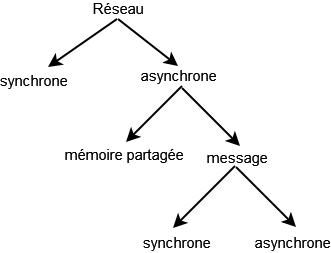
\includegraphics[width=8cm]{figures/algodist.png}
  \caption{Les types des r�seaux en terme de synchronisation, un sch�ma
  pareil peut  �tre �labor� en  s'appuyant sur la connaissance  ou pas
  des noeuds du r�seau}
  \label{fig:algodist}
\end{figure}
\subsubsection{Algorithmique distribu�e}
 La difficult� de  l'algorithmique distribu�e vient essentiellement du
fait  que  chaque  processeur  doit communiquer  uniquement  avec  ses
voisins, � l'aide de registres partag�s, ou par �change de message. De
mani�re g�n�rale,  on d�finit un algorithme distribu�  par un ensemble
de  r�gles  de  transformations  d'�tat  (avec  un  ordre  partiel  de
priorit�).  Si les  transformations induites  par cet  algorithme sont
ind�pendantes, elles sont susceptibles avoir lieu en m�me temps, sinon
on choisit une fa�on non d�terministe la transformation � effectuer.

\subsubsection{Preuve en algorithmique distribu�e}
La preuve d'un tel algorithme se fait en deux temps.  Tout d'abord, on
prouve  la   terminaison  de  l'algorithme,   par  des  consid�rations
combinatoires sur le nombre maximum d'�tapes, qui doit �tre fini. Puis
on   prouve   la  validit�,   le   plus   souvent   en  exhibant   des
invariants... sur lesquels on s'appuie pour r�diger la preuve.
\subsubsection{messages synchrones}
On parle de messages synchrones lorsque l'envoyeur et le receveur sont
synchronis�s, c'est-�-dire  qu'un rendez-vous est mis en  place par un
protocole  (exemple,  le  t�l�phone).  Par  opposition,  on  parle  de
messages  asynchrones  lorsqu'il   y  a  une  d�synchronisation  entre
l'envoyeur et le receveur (exemple, le courrier �lectronique).
%\section{Des principes de base}

\section{Quelques algorithmes simples}
%%%
\subsection{Algorithme de reconnaissance d'un graphe connexe}
On part  d'un sommet que  l'on marque, on  empile ses voisins.  On les
visite,  on les marque  et on  empile les  voisins des  voisins..., Le
graphe est connexe\footnote{Un graphe  (orient� ou non) est connexe si
et  seulement si, pour  tout couple  de sommets,  il existe  une suite
d'ar�tes reliant ces sommets.
\label{grapheConnexe}}  si  tous les  sommets  sont  marqu�s. Pour  la
reconnaissance d'un  graphe fortement connexe,  il convient d'utiliser
deux marques.

\subsection{Algorithme n�1 pour le calcul d'un arbre recouvrant}
Cet  algorithme   permet  le   calcul  d'un  arbre   recouvrant  (sans
reconnaissance locale de la  terminaison globale, cf.  algorithme n�2)
. Consid�rons la r�gle de transformation suivante:

\begin{figure}[ht]
  \centering
  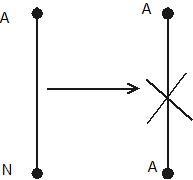
\includegraphics[width=5cm]{figures/algodist1.png}
  \caption{Algorithme n�1: Exemple d'une transformation A-N}
  \label{fig:algodist1}
\end{figure}

On  se donne  un graphe  G. Initialement  tous les  sommets  sont dans
l'�tat Neutre.  On choisit  un premier sommet,  dans l'�tat  Actif. On
applique  les transformations  � partir  de ce  point.  Le sous-graphe
d�fini  par les  ar�tes marqu�es  est  un arbre  recouvrant du  graphe
initial.
\subsection{Algorithme n�2 pour le calcul d'un arbre recouvrant}
Cet algorithme  permet le calcul d'un arbre  recouvrant avec d�tection
locale de la terminaison globale  (�tat F).  Consid�rons les r�gles de
transformation suivantes. R1 a une plus grande priorit� que R2.

\begin{figure}[ht]
  \centering
  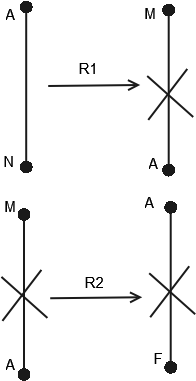
\includegraphics[width=4cm]{figures/algodist2.png}
  \caption{Algorithme n�2  : Exemple d'algorithme � base  de r�gles de
  r��critures}
  \label{fig:algodist2}
\end{figure}

\section{Exemples de probl�mes de l'algorithmique distribu�e}
Dans  le domaine  de l'algorithmique  distribu�es on  trouve  plein de
probl�me qui sont  connus, dans cette partie il  s'agit pas de traiter
ces probl�mes mais juste de donner une id�e sur eux.
\subsection{Le probl�me de l'�lection}
On consid�re  un r�seau ; on  souhaite positionner un  unique noeud du
r�seau dans un �tat �lu et tous les autres dans un �tat non �lu.
\subsubsection{Algorithme dans le cas d'un anneau} 
Soit G un anneau, asynchrone avec �change de messages asynchrones, � 3
�tats :  non �lu,  �lu, ind�fini. Les  sommets sont  initialement dans
l'�tat   ind�finis.  Chaque   processeur  i   du  r�seau   poss�de  un
identificateur   $id_{i}$  unique  (un   entier).  L'anneau   est  orient�,
c'est-�-dire  que  les processeurs  ont  la  notion  de gauche  et  de
droite.   Le  processeur   �lu  est   celui  qui   a  le   plus  grand
identificateur.  Chaque processeur transmet � son voisin de droite son
identificateur. Lorsqu'un processeur re�oit  un identificateur, il y a
trois possibilit�s :
\begin{itemize}
\item Si l'identificateur re�u est plus grand que le sien, il le passe
au suivant (voisin de droite) et passe dans l'�tat non �lu.
\item Si l'identificateur re�u est plus petit que le sien, il jette le
message.
\item Si l'identificateur re�u est le m�me que le sien, alors il prend
l'�tat �lu.
\end{itemize}

\subsection{Probl�mes de reconnaissance}
Peut-on savoir si le r�seau  est un graphe complet, planaire, si c'est
un arbre,  un anneau  ?  Peut-on  savoir encore si  un sommet  est une
articulation, si  une ar�te est un  isthme ?  Dans le  premier cas, il
existe un syst�me de r��criture (ou calcul local) tel que, quand il se
termine, la collecte des  �tiquettes sert de crit�re de reconnaissance
; dans le second cas, ce n'est pas possible !
\subsection{D�tection de la terminaison}
Savoir qu'un protocole distribu� est termin� est souvent difficile. On
peut chercher �  avoir un d�tection locale de  la terminaison globale,
c'est-�-dire qu'un processeur  peut savoir en fonction de  son �tat et
de celui de ces voisins si l'algorithme est termin�.


\section{Quelques applications}
L'algorithmique distribu�e est appliqu� dans plusieurs domaines, Comme
par exemple :
\subsection{Construction d'objets parall�les}
Un exemple des applications dans ce domaine est men� par le PRISM
\footnote{le laboratoire  de recherche en informatique  sur les th�mes
du Parall�lisme, des R�seaux, des Syst�mes et de la Mod�lisation.(voir
http://www.prism.uvsq.fr/)}, il consiste dans la construction d'objets
pour  l'�laboration d'algorithmes  d'alg�bre lin�aire  utilisables par
des architectures � m�moire distribu�e.
\subsection{Le domaine de l'�nergie}
Un  exemple  d'application  dans  ce  domaine  on  le  trouve  au  LAG
\footnote{le Laboratoire    d'Automatique    de   Grenoble    (voir
http://www.lag.ensieg.inpg.fr/)}  ,  et  qui  vise  contrairement  aux
approches  traditionnelles  qui  consistent  � ajuster  la  production
d'�nergie pour  satisfaire �  la demande, �  proposer un  m�canisme de
coop�ration entre sources et charges  de fa�on � satisfaire au mieux �
des crit�res de satisfaction d�finis par un usager. 

\subsection{Autres applications}
L'algorithmique  distribu�e  est pr�sente  partout  o�  on trouve  des
syst�mes   distribu�s,   ces  derniers   sont   devenu  une   solution
incontournable  dans  plusieurs domaines.  Par  exemple  la plupart  des
syst�mes de s�curit�  et de gestion des pannes  utilisent les th�ories
de ce domaine,  ce qui engendre autant de probl�mes  � r�soudre que de
solutions � proposer.


%algorithmique distribu�e
%hicham
\chapter{Analyse de l'existant}
Apr�s avoir  pr�sent� le  domaine de l'algorithmique  distribu�e, nous
allons  maintenant  faire  un  tour  d'horizon  de  l'implantation  de
\visidia telle qu'elle existait avant notre apport. 

\section{But de \visidia}

Comme  nous  l'avons  d�j�  vu,  la  visualisation  et  la  simulation
d'algorithmes distribu�s  est de plus en plus  n�cessaire pour �tablir
de  nouveaux   mod�les,  trouver   de  nouveaux  algorithmes   et  les
prouver. C'est dans cette optique que le projet \visidia a �t� lanc� :
permettre  d'approfondir   les  connaissances  dans   le  domaine  des
algorithmes distribu�s en facilitant la simulation et la visualisation
en temps r�el de leurs ex�cutions.

\section{Repr�sentation des r�seaux}

Dans  \visidia comme  dans beaucoup  de  travaux sur  les r�seaux,  la
repr�sentation �  l'aide de graphes est  utilis�. Cette repr�sentation
permet  d'associer  d'une  fa�on  tr�s  claire  les  syst�mes  ou  les
processeurs � des noeuds du  graphe et leurs connexions aux ar�tes (ou
arcs).\\

Cette   repr�sentation  nous   permet  de   d�crire   les  diff�rentes
caract�ristiques des r�seaux.  Par exemple :\\

\begin{itemize}
\item   les  liaisons  unidirectionnelles   de  notre   r�seau  seront
repr�sent� gr�ce � des arcs sur un graphe orient�,
\item le  poids des ar�tes  repr�sentera les d�lais  d'acheminement de
l'information entre deux syst�mes connect�s etc.
\end{itemize}

\section{Mod�le implant�}

L'algorithmique distribu�e  est une science qui n'a  pas encore trouv�
toutes ses  marques. Il  existe de nombreux  mod�les pour  d�crire les
algorithmes et m�me si certains  de ses mod�les sont plus utilis�s que
d'autres, aucun  n'a encore  montr� de facult�  � supplanter  tous les
autres.

\subsection{Communication par messages}

Le mod�le  choisit pour l'implantation  de \visidia est l'un  des plus
r�pandus : il s'agit de  la communication par messages. Dans ce mod�le
chaque noeud, repr�sentant un syst�me ou un processeur, est habilit� �
ex�cuter  un algorithme. Cet  algorithme poss�de  certaines primitives
qui lui  permettent de communiquer avec les  algorithmes implant�s sur
les  noeuds  voisins.  Il  est  par exemple  possible  �  un noeud  de
demander une synchronisation  avec un ou plusieurs de  ses voisins, de
leur envoyer  des messages, d'en recevoir etc.   Nous d�taillerons ces
primitives dans la section \ref{sec:existant-api}.\\

\subsection{Description de l'API existante}
\label{sec:existant-api}

�tudions quelques une des fonctions les plus utilis�es de l'API.

\begin{description}

\item[sendTo]  Permet d'envoyer  un message  sp�cifique sur  une porte
donn�e.

\item[sendAll] Envoie  un message �  tous les voisins (sur  toutes les
portes).

\item[receiveFrom] Attend de recevoir un message provenant d'une porte
donn�e.

\item[receive] Permet de  recevoir un message qui nous  est destin� et
  la  porte dont  il provient.  L'appel �  cette m�thode  attend qu'un
  message arrive s'il n'y en a pas d�j� un dans la file. 

\item[getArity] Retourne  le degr�  du sommet en  cours (le  nombre de
portes). 

\item[getNetSize] Retourne le nombre de sommet du graphe.

\item[setDoorState]   Modifie   l'ar�te    point�e   par   une   porte
  donn�e. G�n�ralement utilis�e pour mettre une ar�te en gras.

\item[putProperty] Change  une valeur de la table  des propri�t�s d'un
  sommet. Presque uniquement utilis�e pour changer le label d'un somme
  (sa couleur). 

\item[getProperty] R�cup�re une valeur dans la table des propri�t�s du
  sommet.  Presque uniquement  utilis�e  pour conna�tre  le label  (la
  couleur) en cours d'un sommet.

\end{description}

\subsection{Exemple d'utilisation}

Voici un exemple  d'utilisation du mod�le par envoie  de messages pour
calculer un arbre couvrant. A l'origine, tous les sommets ont un label
``N'' sauf  un qui a un  label �gal � ``A''  et qui jouera  le r�le de
racine.

\begin{verbatim}
init() {

  if(getProperty(``label'') = ``A'') {
    sendAll(``Wave'');
  }
  else {
    (message, porteDuPere) := receive();

    setDoorState(MARKED_STATE, porteDuPere); //marque l'ar�te en gras

    putProperty(``label'', ``A'');

    for(i=0 ; i < getArity() ; i++) {
      if (i != porteDuPere) {
        sendTo(i, ``Wave'');
      }
    }
  }
}
\end{verbatim}

Voici l'ordre dans lequel se d�roulent les �tapes :\\

\begin{enumerate}

\item  Tous les  noeuds ``N''  sont en  attente d'un  message  suite �
l'appel de la m�thode $receive$.

\item La racine envoie simplement un message
(contenant  le  mot   ``Wave'')  �  tous  ces  voisins   avant  de  se
terminer. 

\item  Les   voisins  de  la   racine  re�oivent  le  message,  se
  d�bloquent et  marquent l'ar�te de  laquelle provient le  message en
  gras (cette ar�te fera partie de l'arbre couvrant).

\item Ces  sommets jouent  ensuite le r�le  de racine et  renvoient un
  message � tous  leurs voisin (sauf � l'exp�diteur  du message qu'ils
  viennent de  recevoir) puis se terminent. Ceci  d�bloque de nouveaux
  sommets qui vont ex�cuter les �tapes 3 et 4.

\item Quand tous  les sommets se sont termin�s,  l'algorithme est fini
  et un arbre recouvre le graphe.

\end{enumerate}

La preuve de  cet algorithme est facile et se base  sur les deux faits
suivants :\\

\begin{itemize}

\item Un  seul noeud  lance le processus  initial ce qui  implique que
  pour tout noeud du graphe,  il existe un chemin remontant jusqu'� la
  racine. 

\item Chaque noeud marque une et une seule ar�te.

\end{itemize}

\section{Architecture g�n�rale}

Nous allons maintenant nous attarder � d�crire l'architecture g�n�rale
du programme \visidia.\\

\visidia se base sur trois grandes structures :\\

\begin{itemize}

\item l'interface graphique
\item le simulateur
\item les algorithmes

\end{itemize}

\subsection{Interface graphique}

L'interface graphique est une  partie tr�s importante de l'application
\visidia. C'est  gr�ce �  elle que \visidia  a beaucoup de  succ�s. En
effet,  elle permet  de visualiser  en temps  r�el le  d�placement des
messages sur le graphe et l'�tat des sommets.\\

L'interface graphique se compose de  deux parties : la premi�re partie
est  consacr�e � l'�dition  de graphe  et la  seconde �  la simulation
proprement dite.

\subsubsection{Interface graphique d'�dition}

Dans la partie consacr�e  � l'�dition, l'interface graphique permet de
cr�er de nouveaux graphes par la seule utilisation de la souris. Gr�ce
� elle, de simples glisser/d�poser permettent de placer des sommets et
de les relier par des ar�tes.\\

Cette interface permet aussi de  charger des graphes existants, de les
compl�ter\dots

\subsubsection{Interface graphique de simulation}

La partie la plus int�ressante de l'interface graphique se trouve dans
la fen�tre de simulation. De nombreuses t�ches peuvent �tre effectu�es
dans cette partie parmis lesquelles :\\

\begin{itemize}

\item charger un algorithme et le placer sur les sommets du graphe,
\item lancer la simulation, la mettre en pause et l'arr�ter,
\item voir en temps r�el les messages s'�changer sur les ar�tes,
\item choisir des r�gles de r��criture � appliquer,
\item �diter les labels des sommets\dots

\end{itemize}

\subsection{Simulateur}

Le simulateur est  le noyau de \visidia. Il a  entre autre pour charge
de :\\

\begin{itemize}
\item lancer l'ex�cution des algorithmes,
\item g�rer les messages du r�seau,
\item informer l'interface graphique des changements,
\item valider les acquittements de l'interface graphique,
\item compter les �v�nements en vue d'�tablir des statistiques\dots
\end{itemize}

\sauteligne

Lorsque le simulateur est cr�� par l'interface graphique, celle-ci lui
fournit  le  graphe  courant,  l'algorithme  �  ex�cuter  choisit  par
l'utilisateur  et deux files  qui serviront  � la  communication (voir
\ref{sec:existant-communication}). Le simulateur se charge � ce moment
d'initialiser les  files de messages pour les  algorithmes. Mais c'est
au moment  o� le  simulateur re�oit un  appel �  $startSimulation$ que
celui-ci commence  r�ellement son travail.   Il va cr�er,  pour chaque
noeud du graphe, un processus  qui va ex�cuter le code de l'algorithme
s�lectionn�.\\

Par la  suite, le r�le  du simulateur sera  de g�rer les  demandes des
algorithmes  (informations sur  le graphes,  envoies et  r�ceptions de
messages\dots) et de l'interface graphique (mise en pause ou � l'arr�t
du simulateur\dots).

\subsection{Algorithmes}

Les algorithmes repr�sentent la  partie �volutive de \visidia. Pour se
servir  de  \visidia,  l'utilisateur  devra commencer  par  �crire  un
algorithme en Java  en utilisant l'API fournie (il  est aussi possible
de dessiner  des r�gles  de r��critures, nous  en reparlerons  dans la
partie \ref{sec:existant-reecriture}).\\

Lors   du   lancement  de   l'algorithme,   la   m�thode  $init$   est
appel�e.  C'est  cette  m�thode  que l'utilisateur  de  \visidia  doit
implanter. Elle est g�n�ralement �crite de la fa�on suivante :

\begin{verbatim}
init() {

 // Partie d'initialisation

  while(true) {

    // M�canisme de synchronisation avec un ou plusieurs voisins

    // Envoies et r�ceptions de messages

    // Changement de l'�tat du sommet et/ou d'une ar�te

    // Quitter la boucle sous certaines conditions

  }

}
\end{verbatim}

Les algorithmes  ne peuvent rien  faire tout seul. Toutes  les actions
qu'ils veulent  entreprendre, comme l'envoie de  messages, passent par
le simulateur.\\


\subsubsection{Gestion de l'arr�t d'un algorithme}

Un algorithme  peut se terminer de  deux fa�ons diff�rentes  : soit il
n'a plus rien � faire et la m�thode $init$ se termine simplement, soit
l'utilisateur demande  explicitement l'arr�t du simulateur  qui va lui
m�me interrompre  les algorithmes. C'est cette  deuxi�me technique que
nous allons aborder ici.\\

Mettre en place un m�canisme d'interruption propre des processus en Java
passe  une  gestion  fine   des  exceptions.   Lorsque  l'on  souhaite
interrompre  un  processus, il  est  n�cessaire  de  lui appliquer  la
m�thode  $interrupt$.  Cela  dit,  cette m�thode  n'interrompt  pas  �
proprement parler le processus. Deux  cas peuvent se pr�senter lors de
l'appel � cette m�thode :

\begin{itemize}
\item le processus est actif, auquel cas la m�thode $interrupt$ n'aura
  aucun effet et le processus continuera son activit�,
\item le processus est en  attente d'un �v�nement (typiquement suite �
  l'appel   �    la   m�thode    $wait$)   auquel   cas    un   signal
  $InterruptedException$ lui est envoy�.
\end{itemize}

Les  d�veloppeurs de \visidia  ont d�cid�  de capturer  les exceptions
$InterruptedException$     pour      les     remplacer     par     des
$SimulationAbortError$ qui  ne sont jamais captur�es  et qui terminent
donc  le processus  qui  a re�u  le  signal.

\subsection{Communication entre les structures}
\label{sec:existant-communication}

Dans  cette partie  nous d�crirons  bri�vement comment  les structures
communiquent entre elles.

\begin{figure}[ht]
  \centering
  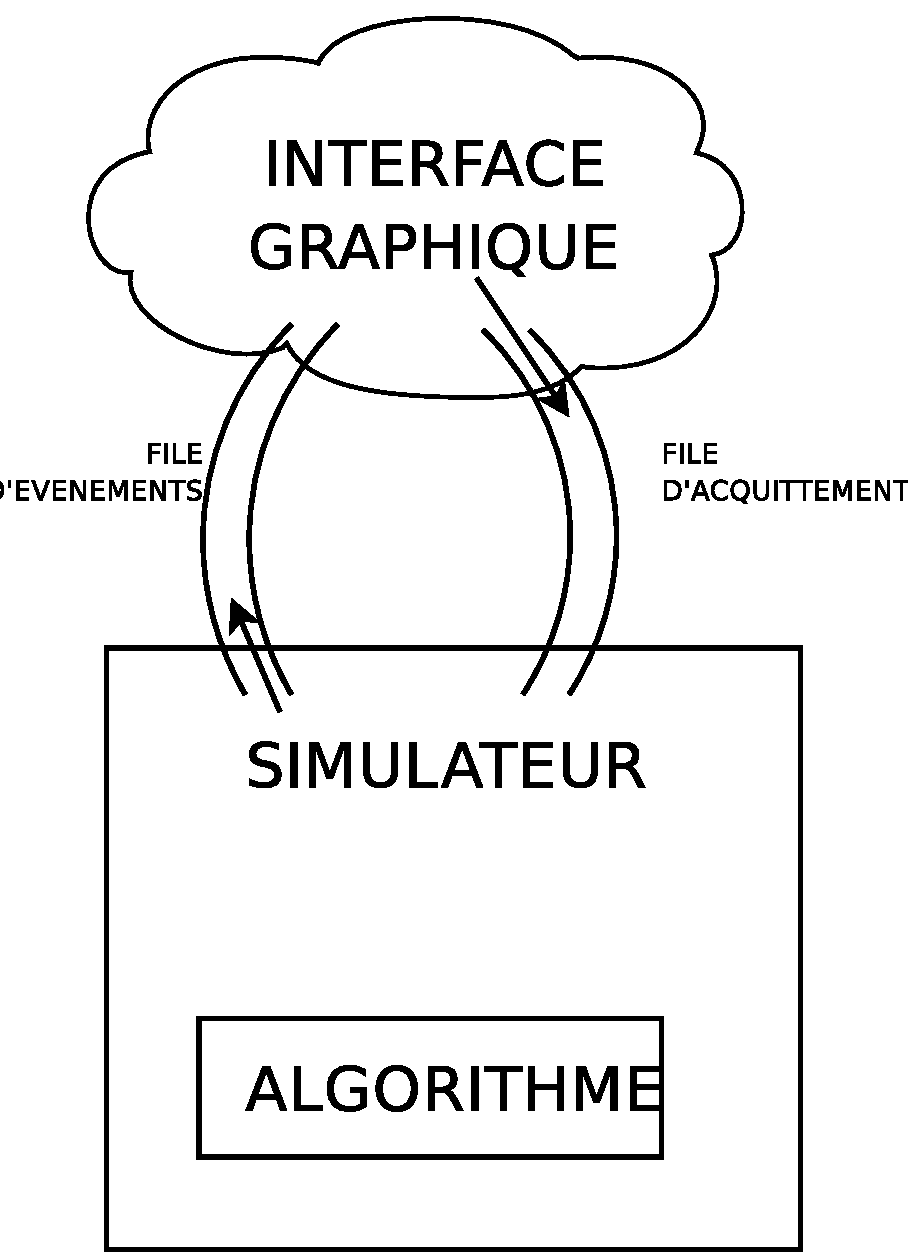
\includegraphics[width=6cm]{existant-communication}
  \caption{Communication entre les structures}
  \label{fig:existant-communication}
\end{figure}

\subsubsection{Entre la partie graphique et le simulateur}

\subsubsection{Entre les algorithmes et le simulateur}

\section{Modes d'utilisations}
\subsection{Syst�me unique}
\subsection{Distribu�}
\subsection{R�gles de r��criture}
\label{sec:existant-reecriture}


\section{Limite du mod�le actuel}

\section{Un nouveau mod�le : les Agents}

%% Local Variables: 
%% mode: latex
%% TeX-master: "rapport"
%% TeX-PDF-mode: t
%% coding: latin-1
%% End:
%ViSiDiA + autres simulateurs AD�gents
%damien
\chapter{Pr�sentation du projet}
\section{Le projet}

\subsection{Le sujet du projet}

\visidia est un logiciel permettant de visualiser et de simuler des
algorithmes distribu�s. Le mod�le actuellement utilis� consiste �
impl�menter un processus pour chaque sommet du graphe consid�r�. Un
sommet peut communiquer uniquement avec ses voisins par envois de
messages. Le logiciel permet, gr�ce � l'interface graphique de
visualiser l'�tat de chaque sommet ainsi que les messages re�us et
�mis.\\ Ce mod�le d'implantation des algorithmes distribu�s est tr�s
utilis�, le d�veloppement d'un logiciel permettant sa simulation �tait
n�cessaire et a d�j� fourni de nombreux r�sultats. N�anmoins, la
simulation de ce mod�le a des limites, notamment pour la simulation de
grands graphes. \\

L'objectif de ce projet est donc de concevoir et d�velopper une
version utilisant uniquement des entit�s mobiles de calcul, appel�es
agents mobiles. Dans ce mod�le, ce ne sont plus les sommets du graphe
qui ex�cutent un algorithme, mais les agents. Ceux-ci se d�placent sur
le graphe et ex�cutent un algorithme selon leurs propri�t�s et celles
du sommet sur lequel ils se trouvent.

\subsection{Le cadre}

Ce projet se d�roule dans le cadre du PFA \footnote{Projet de Fin
d'Ann�e}.  D'une dur�e de 4 mois, il s'int�gre dans la formation
d'ing�nieur � l'ENSEIRB.  Il a pour but de familiariser les �l�ves
avec les m�thodes de travail en �quipe sur des projets de plus grande
taille et de plus longue dur�e.  Ce projet est �galement l'occasion
pour les �l�ves d'�tablir une v�ritable relation avec le client, pour
pouvoir satisfaire � ses besoins.

\subsection{L'�quipe}

Notre �quipe est constitu�e de 7 personnes : Nada Ayad, Damien Cassou,
Xavier Durand, Jean-Baptiste Gautron, Hicham Ghriss, Mathieu Hopmann
et Julie Quagliozzi. Nous avons la particularit� d'avoir une �quipe
tr�s h�t�rog�ne, avec une participation f�minine. De plus, tous les
parcours scolaires sont repr�sent�s. Parmi nous, on peut compter des
personnes venant des classes pr�paratoires, d'IUT et de l'universit�.

\section{L'organisation}

\subsection{Les moyens techniques}

Ce projet a �t� l'occasion d'utiliser un portail �volu� de
d�veloppement, sur le mod�le du portail SourceForge
\cite{SourceForge}.  Nous avons choisi le portail berliOs.de
\cite{berliOs}, pour des raisons de rapidit� des serveurs. Ce portail
met � notre disposition de nombreux outils pour le d�veloppement de
projets.\\ Nous disposons tout d'abord d'une page d'accueil
\cite{visidiaPFA} qui est un Wiki \cite{wiki}. Cette page d'accueil
est divis�e en trois parties, pour les d�veloppeurs, les clients et le
responsable p�dagogique. Dans chaque partie, sont r�unis les liens
vers les outils propos�s par le portail ainsi que des documents
consultables par chacun, � savoir les comptes rendus de r�union et la
derni�re version du cahier des charges.\\
\begin{figure}[ht]
  \centering
  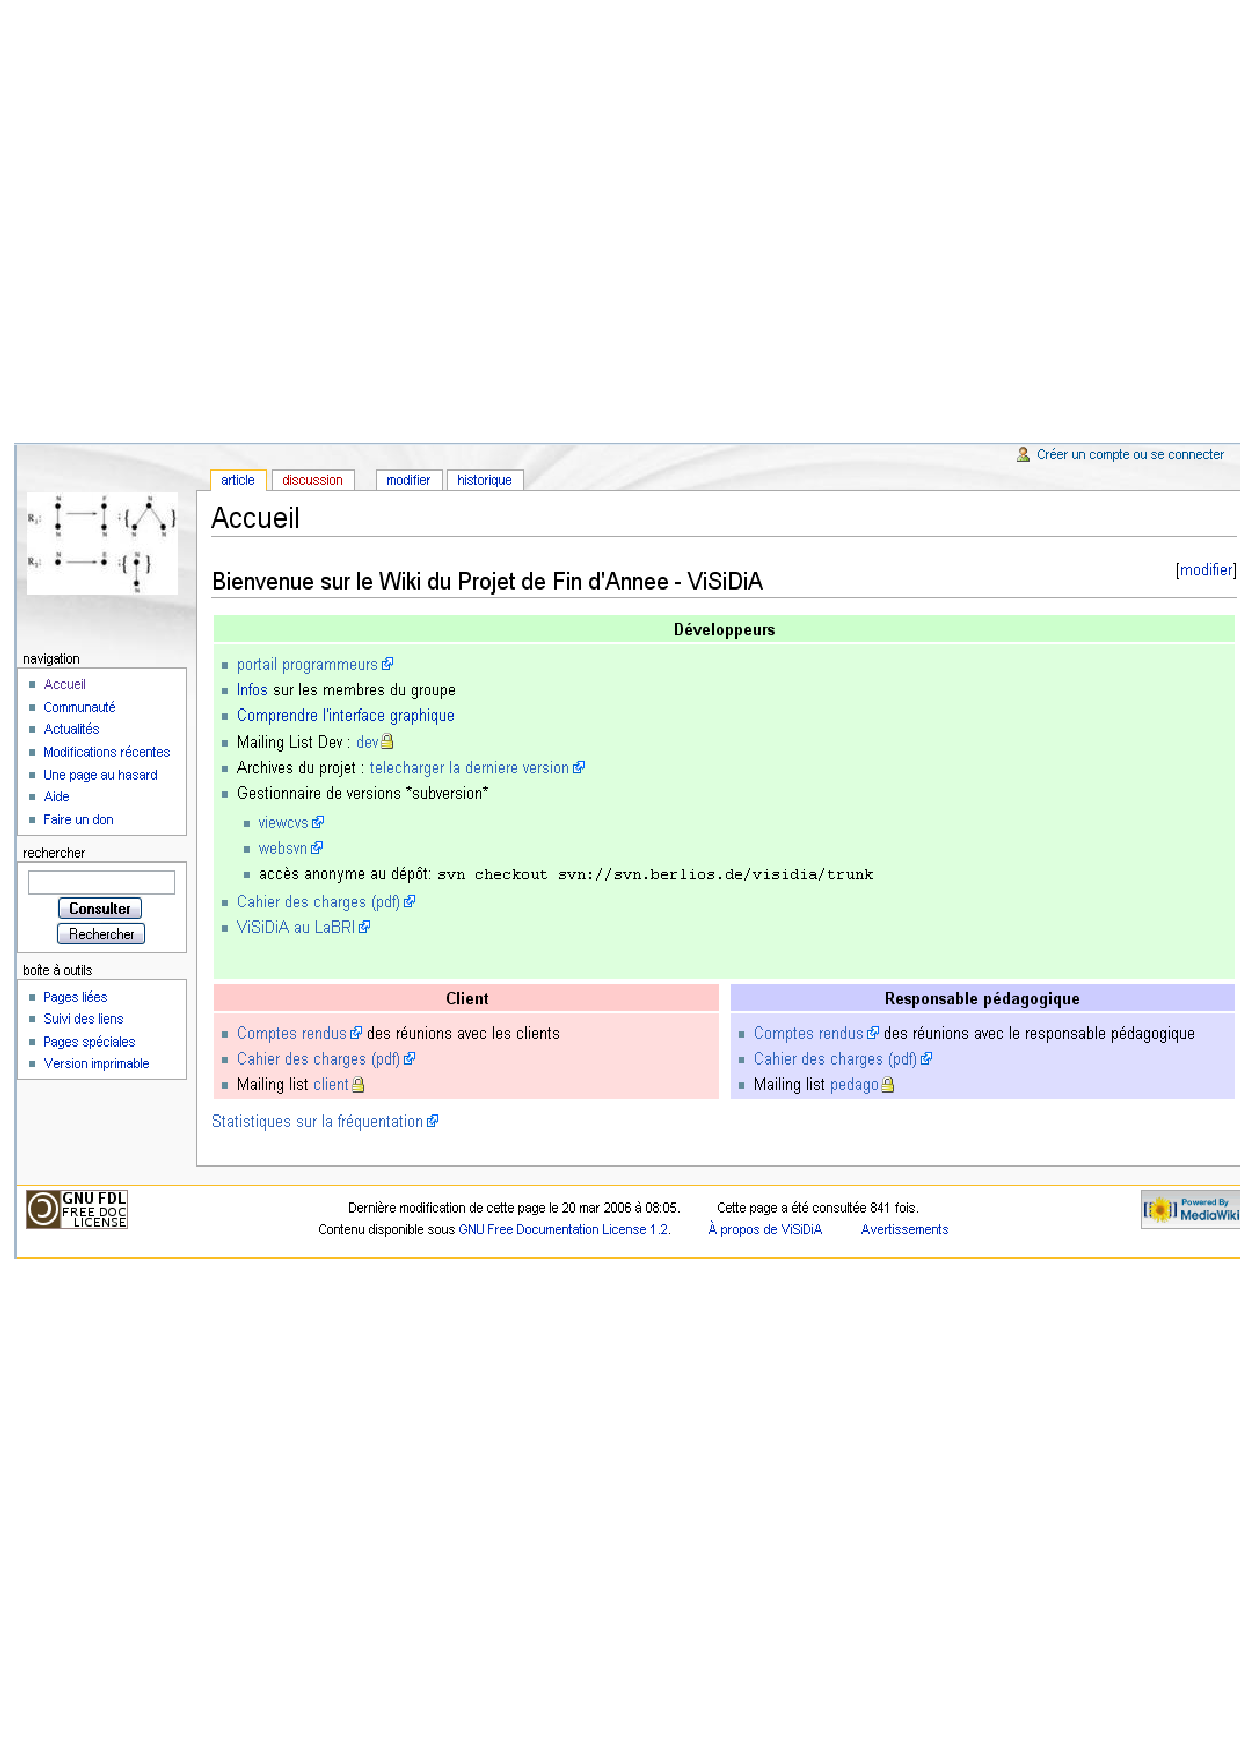
\includegraphics[width=12.5cm]{accueil}
  \caption{page d'accueil de \visidia}
  \label{fig:existant-edition}
\end{figure}

Nous utilisons �galement un gestionnaire de versions, Subversion
\cite{subversion}, qui nous permet de maintenir les sources de notre
extension de \visidia. Les clients ont �galement la possibilit� de
suivre l'avancement du projet et acc�der aux sources, gr�ce � deux
interfaces viewcvs \cite{viewcvs} et websvn \cite{websvn}.  Il est
�galement possible de t�l�charger la derni�re version des sources du
projet:
\begin{verbatim}
svn checkout svn://svn.berlios.de/visidia/trunk
\end{verbatim}
Nous avons �galement mis en place 3 listes de diffusion, une liste
pour les d�veloppeurs, une liste pour les communications avec les
clients, ainsi qu'une liste pour les communications avec le
responsable p�dagogique. Ces listes sont g�r�es par le portail
\berlios.  Il est possible de consulter les archives de ces listes, �
partir de la page d'accueil.

\subsection{Les r�unions}

Nous avons choisi de rencontrer les clients une fois par semaine.
L'horaire du vendredi matin �10h a �t� retenu pour cette entrevue
hebdomadaire. Ces r�unions ont �t� l'occasion de pr�senter aux clients
le travail effectu� et de prendre connaissance des suggestions et
demandes exprim�es par le client. Lors de la plupart de ces r�unions,
toute l'�quipe �tait pr�sente. Lors de chacun de ces entretiens, une
personne �tait charg�e de prendre des notes et r�diger un compte
rendu.  Cette personne �tait volontaire et toujours diff�rente d'un
entretien � l'autre.\\

Les rencontres avec le responsable p�dagogique ont �t� moins fr�quentes,
essentiellement pour pr�senter l'�tat d'avancement du travail. Lors de
ces r�unions ont �t� �galement r�dig�s des compte rendus. Tous ces
comptes rendus sont consultables � partir de la page d'accueil du
projet.

\subsection{L'organisation du travail}

On peut diviser le travail en deux grandes phases, une phase de
conception et une phase de r�alisation. Nous avons choisi de
travailler ensemble tous sur la conception. En effet, cette phase
�tant essentielle au projet, nous avons jug� n�cessaire de r�fl�chir
ensemble sur cette partie. \\ Pour cela, nous avons organis� des
r�unions, lors desquelles nous avons pu discuter des besoins attendus
par le client et voir ainsi si nous avions tous compris la m�me
chose. Lors de ces r�unions, nous pouvions confront� nos points de vue
et nos id�es, face aux questions techniques que nous pouvions
rencontrer. \\

Par la suite, plus particuli�rement lors de la phase de d�veloppement,
ces r�unions �taient l'occasion de faire le point sur l'avancement du
projet, et de se r�partir les t�ches. Il �tait fait un r�capitulatif
des t�ches accomplies et � accomplir lors de la p�riode suivante. La
r�partition des t�ches s'est faite par groupe de 1, 2 ou 3 pour les
plus importantes, en essayant de satisfaire en d�sirs de chacun. On
peut tout de m�me ajouter que cette r�partition s'est faite de telle
sorte que chaque membre de l'�quipe � pu travailler sur l'interface
graphique.

\subsection{L'�ch�ancier}

Un diagramme de Gantt \ref{fig:gantt} planifie les grandes �tapes de
la r�alisation du projet. Ce diagramme �tabli au d�but du projet �
permis d'�tablir les diff�rentes t�ches � r�aliser, et de suivre
l'avancement du projet.\\

\begin{figure}[h!t]
  \centering
  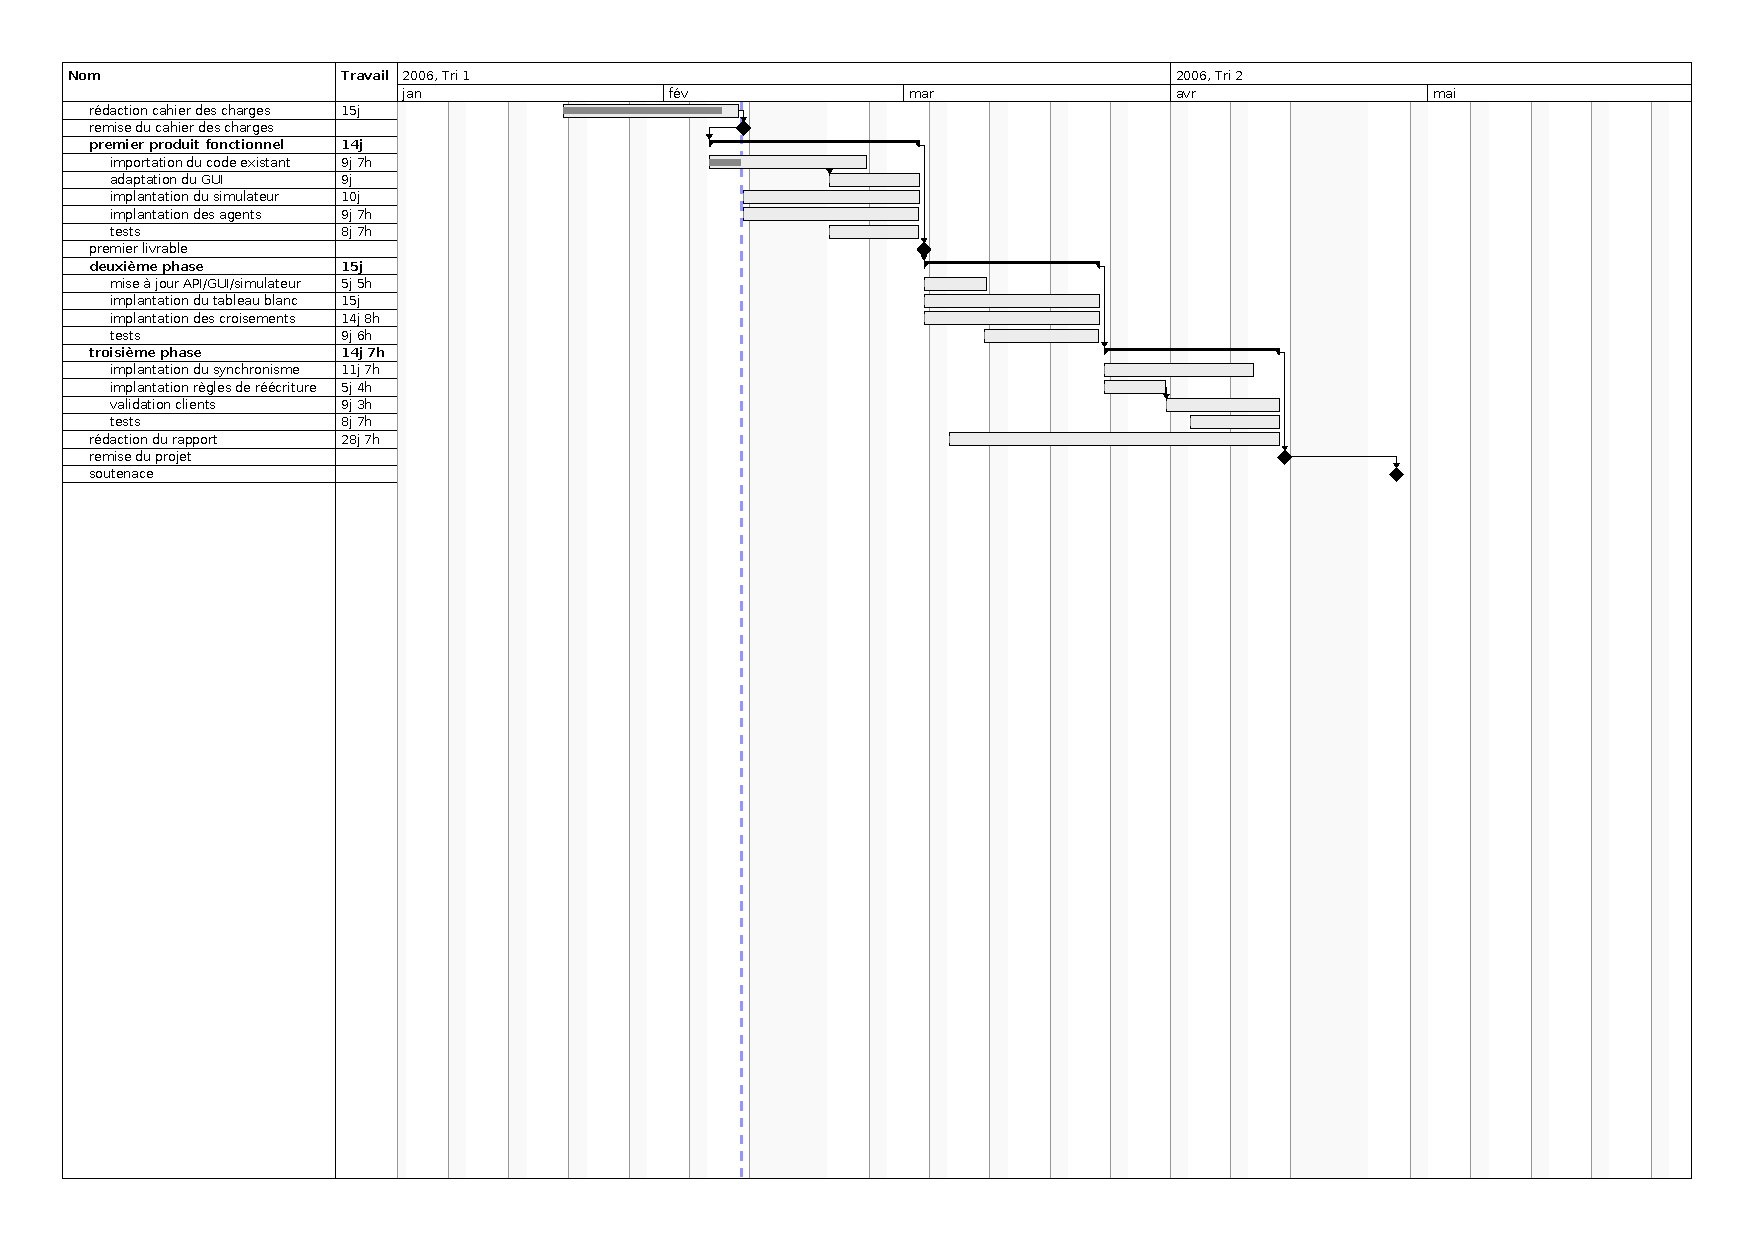
\includegraphics[width=14cm]{gantt}
  \caption{Sc�nario de d�placement}
  \label{fig:gantt}
\end{figure}



La date de remise des sources du projet aux clients a �t� fix�e au
vendredi 14 avril, 17h00 derni�re limite. 

La remise du projet donnera lieu � une soutenance dont la date est
fix�e au jeudi 27 avril.

%- sujet du projet officiel
%- cadre (pfa, enseirb, ingenieur)
%- presentation de l'equipe (fille, prepa, iut, etudiants d'universite)
%- reunions
%- site web/svn
%- organisation dans le code source (packages supplementaires)
%- moyens de communications (wiki/mailing listes)
%- dates (cahier des charges, livrables...) 
%- detailler les livrables prevus/effectifs
%- diagramme de gant

%% Local Variables: 
%% mode: latex
%% TeX-master: "rapport"
%% TeX-PDF-mode: t
%% coding: latin-1
%% End:
%ViSiDiA/agents
%julie
\chapter{Besoins non fonctionnels}
%\input{besoinsNF}
%jb
\chapter{Besions fonctionnels}
%API
%jb
\chapter{Implantation}
Dans cette  partie, nous  allons nous attacher  � d�velopper  de facon
d�taill�e l'implantation de notre  module au sein du logiciel \visidia
existant.\\

Le projet s'est subdivis� en deux parties essentielles :
\begin{itemize}
\item le d�veloppement de l'API et de la simulation.
\item  l'int�gration  des  nouvelles  fontionnalit�s  dans  la  partie
graphique de \visidia.
\end{itemize}


\section{Agents}
Cette section  concerne le d�veloppement  des agents et donc  de l'API
fournie aux clients. Le description  de cette API ayant d�j� �t� faite
dans la  partie pr�c�dente  nous ne nous  attarderons pas  dessus ici.
Elle est  enti�rement d�finie et  implant�e dans la  classe Agent.java
qui se trouve dans  le package visidia.simulation.agents. 

Les m�thodes de cette classe sont bas�es sur des appels au m�thodes du
simulateur qui correspondent.  En effet, comme c'est le simulateur qui
fait le lien  entre l'interface graphique et les agents  il est tout a
fait normal qu'il ait la charge des actions effectu�es par les agents.

En plus  du simlateur  duquel il  d�pend et de  son idetit�,  un agent
contient une  struture de  donn�e de type  WhiteBoard d�finie  dans le
package visidia.tools.agents  et qui permet  � l'agent de  stocker des
informations durant son ex�cution.  Un WhiteBoard s'utilise de la m�me
mani�re qu'une table de  hachage, la diff�rence �tant qu'un WhiteBoard
permet un acc�s a des valeurs par d�faut
\section{Simulateur}


\section{GUI}





%% Local Variables: 
%% mode: latex
%% TeX-master: t
%% TeX-PDF-mode: t
%% coding: latin-1
%% End:
%Structures
%nada
\chapter{Limites de l'implantation}

\section{Lisibilit� et extensibilit�}

Cette  partie ne concerne  pas directement  la simulation  des agents,
mais \visidia dans  son ensemble : le programme souffre  de son �ge et
du fait d'�tre pass� entre de nombreuses mains d'�l�ves ing�nieurs peu
exp�riment�s (y compris nous).\\

De ce fait, il r�sulte  un programme qui fonctionne correctement, mais
aux possibilit�s  d'extension faibles (peu  d'utilisation du m�canisme
d'h�ritage). Ainsi,  les rajouts se greffent directement  dans le code
existant,  ou  via  des   copier-coller,  augmentant  les  risques  de
plantages et/ou d'incoh�rences.\\

Les parties sur  lesquelles nous avons travaill� accusant  ce genre de
probl�me sont  l'interface graphique principalement,  et le simulateur
dans une moindre mesure.

Id�alement,  l'interface  graphique  devrait  permettre le  rajout  de
modules sans avoir � modifier le code d'origine. Malheureusement, pour
cela, une refonte du  code de l'interface graphique semble in�vitable,
or il  s'agit d'un processus  lourd en temps  et personnes, ce  qui le
rend peu envisageable.

Concernant le simulateur, une factorisation des diff�rents simulateurs
existants   serait   pr�f�rable.    Cette  factorisation   n'est   pas
essentielle actuellement mais le  deviendra si d'autres simulateurs se
greffent plus tard � ceux existants.

\section{Simulation sur des graphes de grandes tailles}

Permettre  une visualisation  graphique est  un avantage  certain pour
mieux comprendre et v�rifier le comportement d'un algorithme. Mais une
fois  que le  nombre de  noeuds d'un  graphe d�passe  la  centaine, il
devient  difficile  de  suivre  correctement  le  d�roulement  de  cet
algorithme.\\

Il  s'agit  donc  d'une   limitation  importante,  les  chercheurs  ne
souhaitant  pas  limiter leurs  exp�rimentations  sur  des graphes  de
petite  taille. La  solution  � adopter  pourrait  �tre d'utiliser  le
simulateur  sans passer par  l'interface graphique  puis d'enregistrer
chaque   action  dans  un   fichier,  mais   on  perd   clairement  en
visualisation.

\section{Choix du nombre d'agent}

Utiliser des  agents pour simuler des  algorithmes distribu�s pr�sente
l'avantage  de  pouvoir contr�ler  le  nombre  de  processus qui  sont
ex�cut�s  lors de  la simulation  (contrairement �  la  simulation par
messages qui impose un processus par sommet du graphe).
Le nombre  de processus d�pend en  effet du nombre d'agents  et non du
nombre de sommet. \\

Cet avantage a aussi son inconv�nient : ce que l'on gagne en ressource
machine,  on  le  perd  bien  souvent en  temps  lors  de  l'ex�cution
d'algorithmes  distribu�s  avec  un  faible nombre  d'agents.   Si  au
contraire on souhaite  faire tourner un grand nombre  d'agents, on est
rapidement  limit�  par les  ressources  de  la  machine �  partir  de
quelques milliers d'agents.

Toutefois, cette  flexibilit� reste avant tout un  avantage malgr� ces
limites.

\section{Ajouter des agents apr�s le d�part de la simulation}

Dans  l'�tat actuel  des choses,  l'ajout d'agents  sur le  graphe par
l'utilisateur ne se fait qu'avant le d�part de la simulation. Une fois
que  l'utilisateur a  appuy�  sur le  bouton  start, il  ne peut  plus
ajouter  de nouveaux  agents  au graphe,  seuls  les agents  eux-m�mes
peuvent cr�er d'autres agents (ou se cloner).

%%% Local Variables: 
%%% mode: latex 
%%% TeX-master:  "rapport" 
%%% TeX-PDF-mode: t 
%%% coding:latin-1 
%%% End:

%mathieu
\chapter{Extensibilit�}
%agents sur architecture distribu�e
%gros graphes
%r�gles de r�ecritures
%hicham
\chapter{Exemples de fonctionnement}
\paragraph{Fonctionnement}

Cette partie va illustrer ce rapport d'un jeux de copies d'�crans
rcapitulant les fonctionnalit�s implant�es.

La premi�re �tape � r�aliser est l'�criture de l'algorithme (voir
le Manuel d'utilisation) et sa compilation en bytecode Java.

L'�tape suivante est la cr�ation du graphe sur lequel la simulation va s'effectuer.

\begin{figure}[ht]
  \centering
  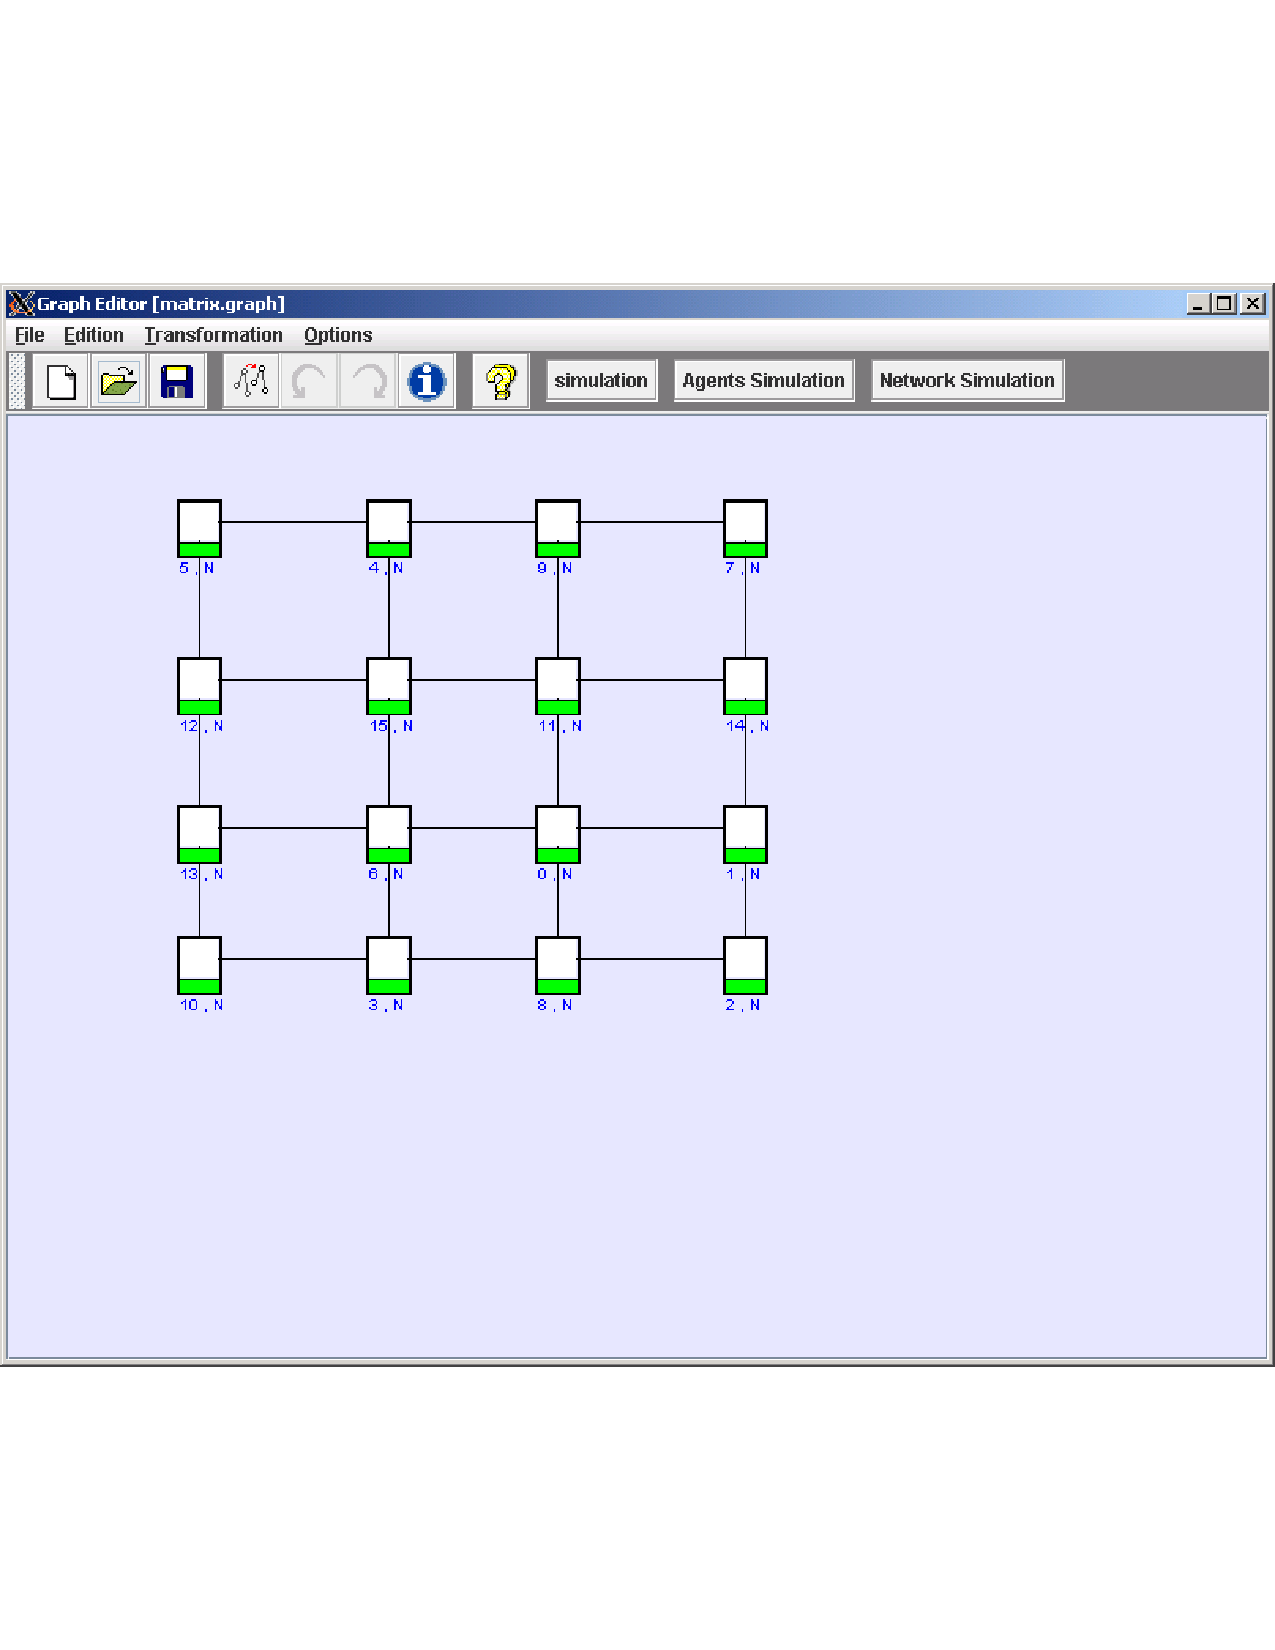
\includegraphics[width=10cm]{fonctionnement-matrix-graph}
  \caption{Fenetre d'edition d'un graph : une grille 4x4}
  \label{fig:fonctionnement-matrix-graph}
\end{figure}

Une fois fois le graphe cr��, la fenetre de simulation peut-etre
lanc�e. A cette �tape, nous ajoutons des agents sur des sommets de
d�part que l'on choisi par s�lection ou par algorithme.

\begin{figure}[ht]
  \centering
  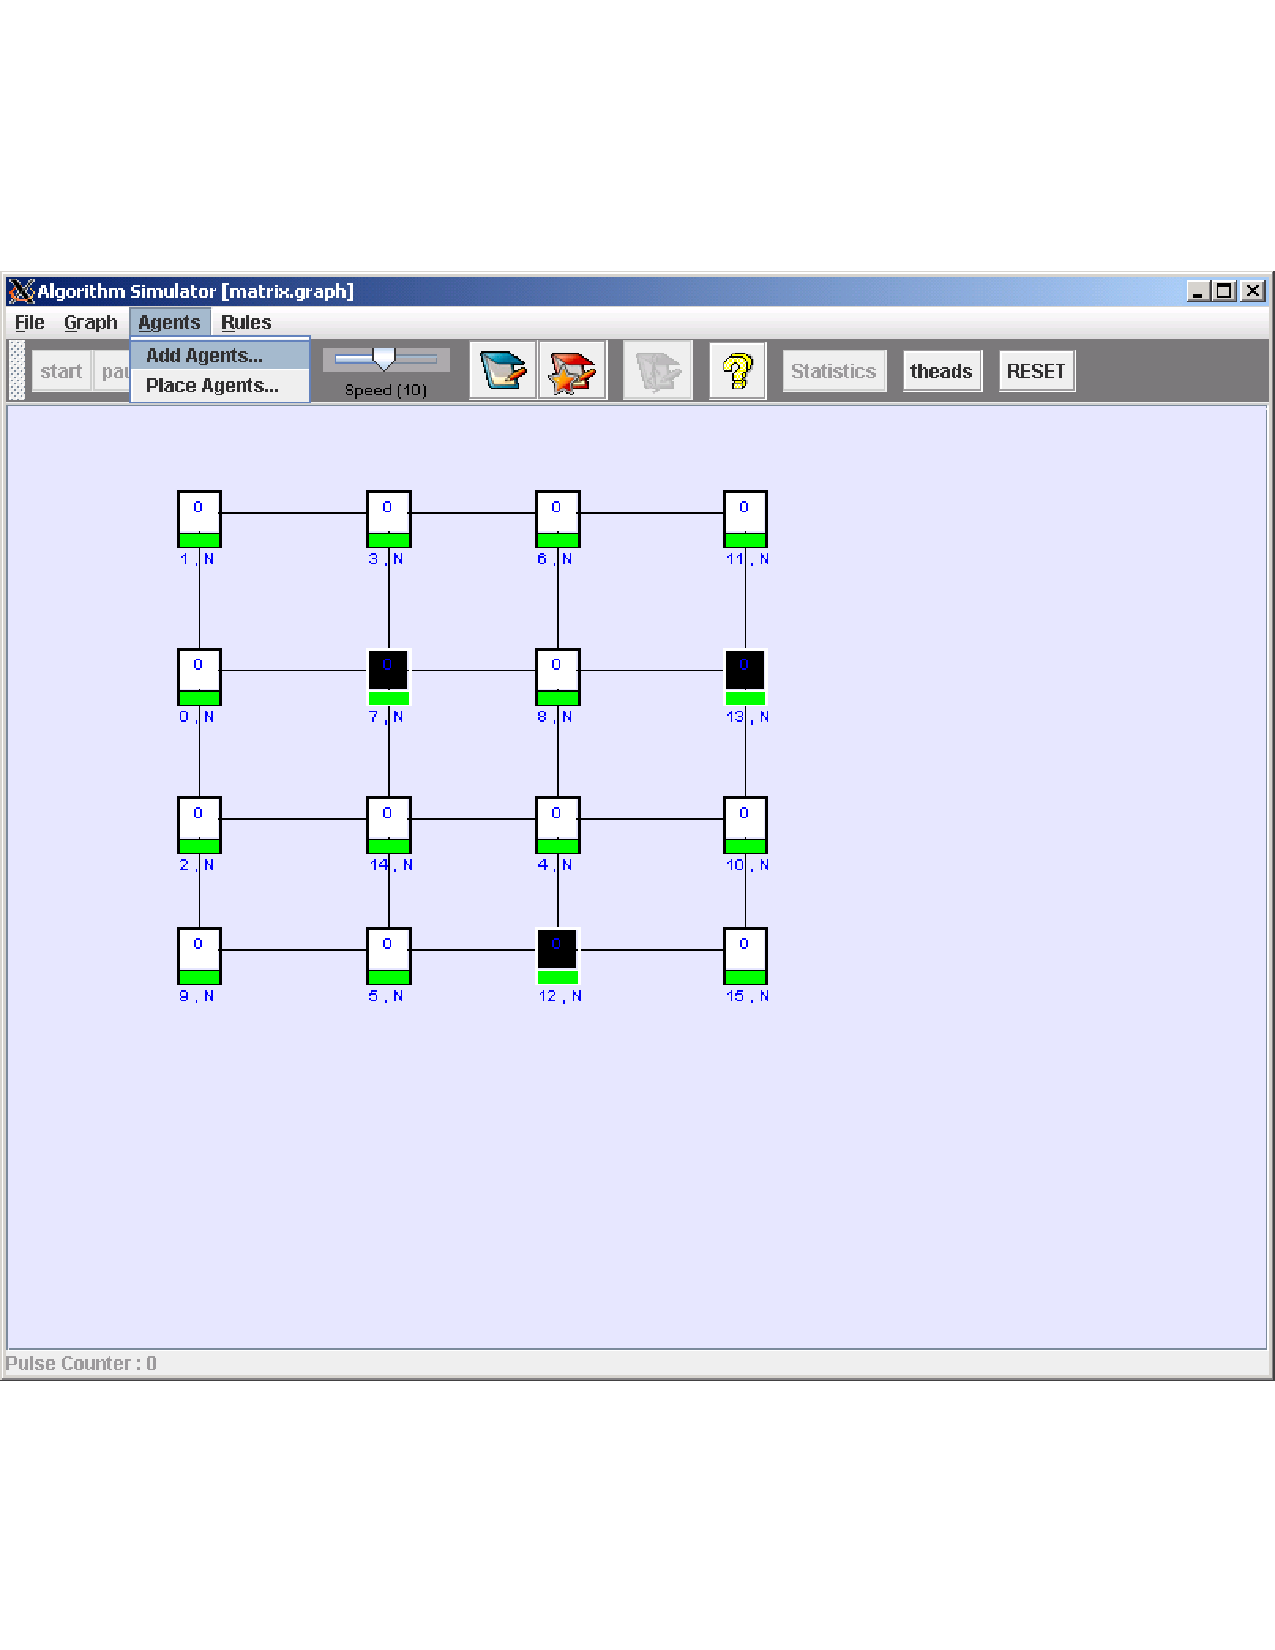
\includegraphics[width=10cm]{fonctionnement-ajout-agent}
  \caption{Ajout d'un type d'agent sur les trois sommets s�lectionn�s}
  \label{fig:fonctionnement-ajout-agent}
\end{figure}

La quatri�me �tape consiste � choisir notre agent compil� dans la
fenetre de s�lection.

\begin{figure}[ht]
  \centering
  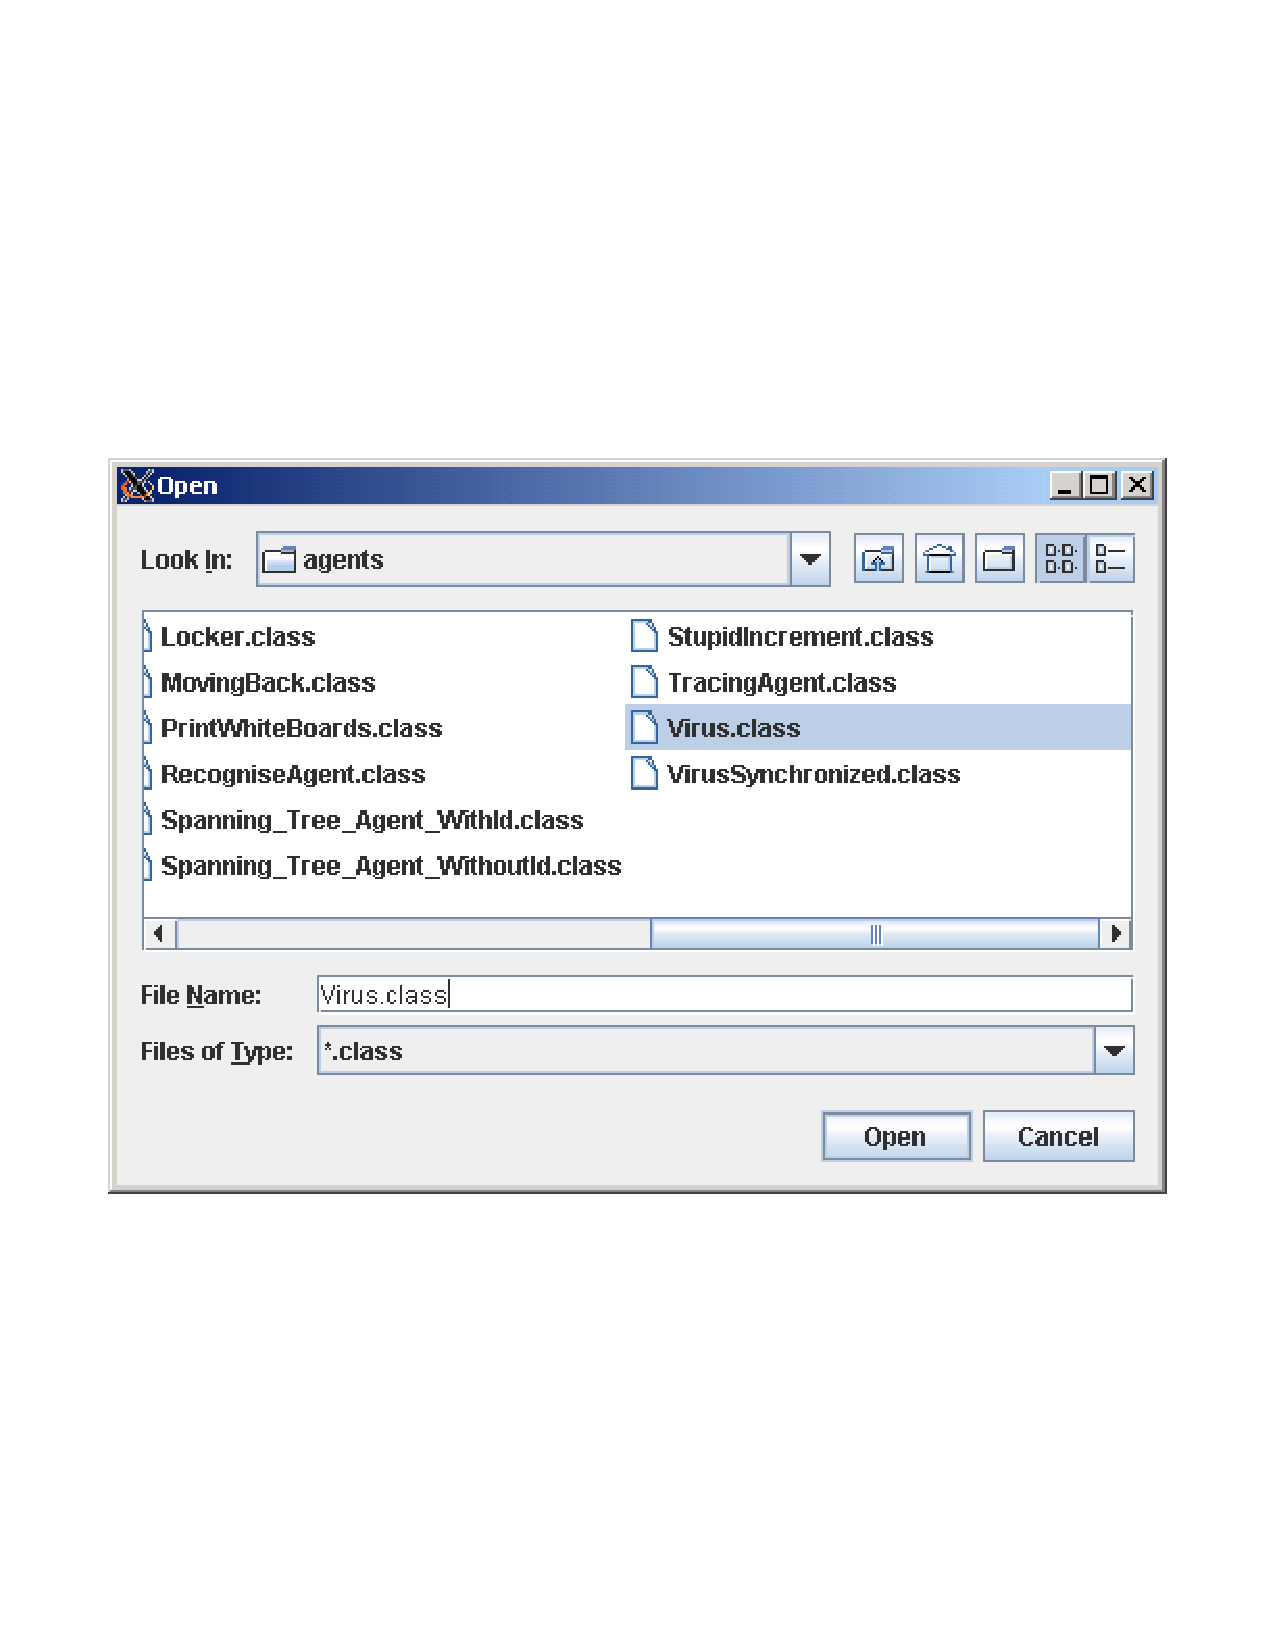
\includegraphics[width=10cm]{fonctionnement-choix-agents}
  \caption{Selection du type d'agent voulu}
  \label{fig:fonctionnement-choix-agents}
\end{figure}

Ensuite vient l'�tape de la simulation proprement dite. Les agents se
d�placent, marquent des aretes, se clonnent ou se suicident
conform�ment � ou aux l'algorithmes d'agent que l'on vient de
programmer. Ces actions sont repr�sent� graphiquement dans la fenetre
de simulation.

\begin{figure}[ht]
  \centering
  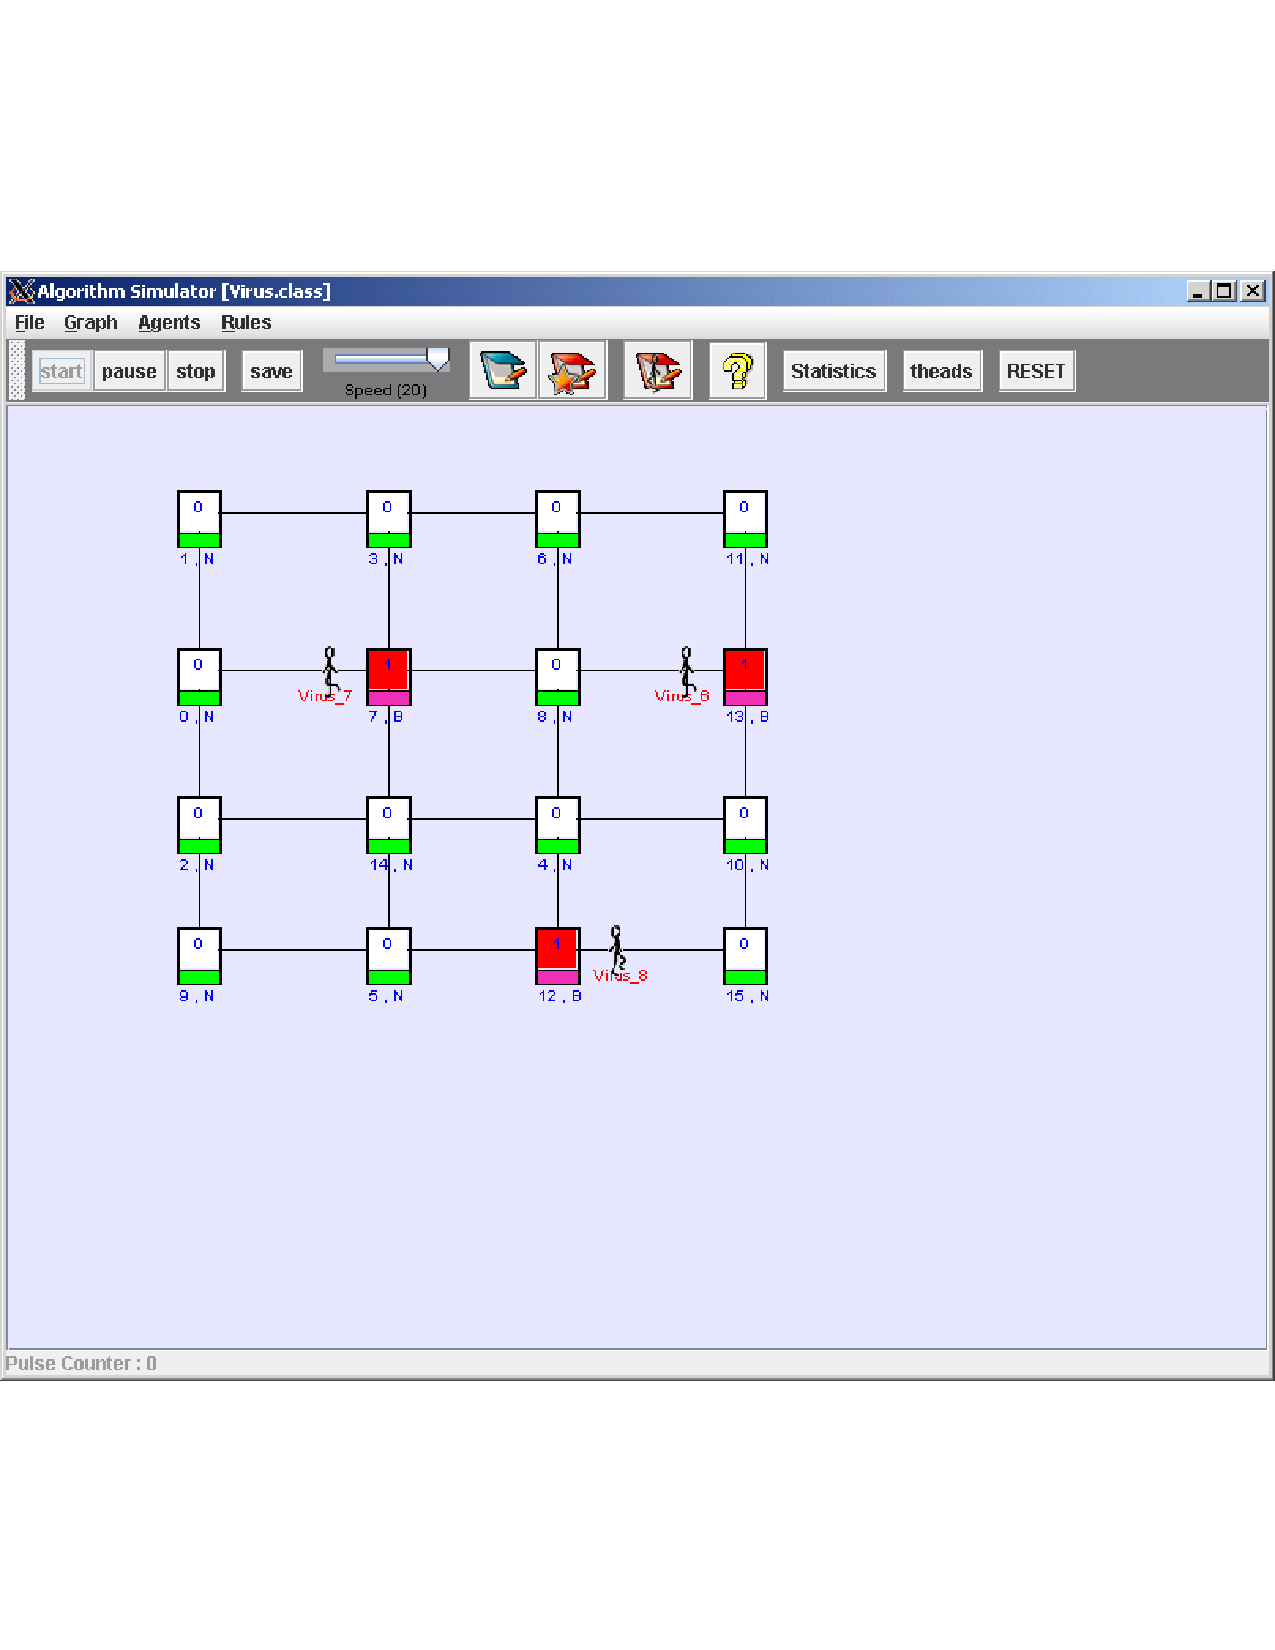
\includegraphics[width=10cm]{fonctionnement-simu1}
  \caption{Simulation en cours : les agents se d�placent sur le graph}
  \label{fig:fonctionnement-simu1}
\end{figure}

On peut �galement visualiser et �diter les whiteboards des agents et
des sommets au cours de la simulation en temps r�el.

\begin{figure}[ht]
  \centering
  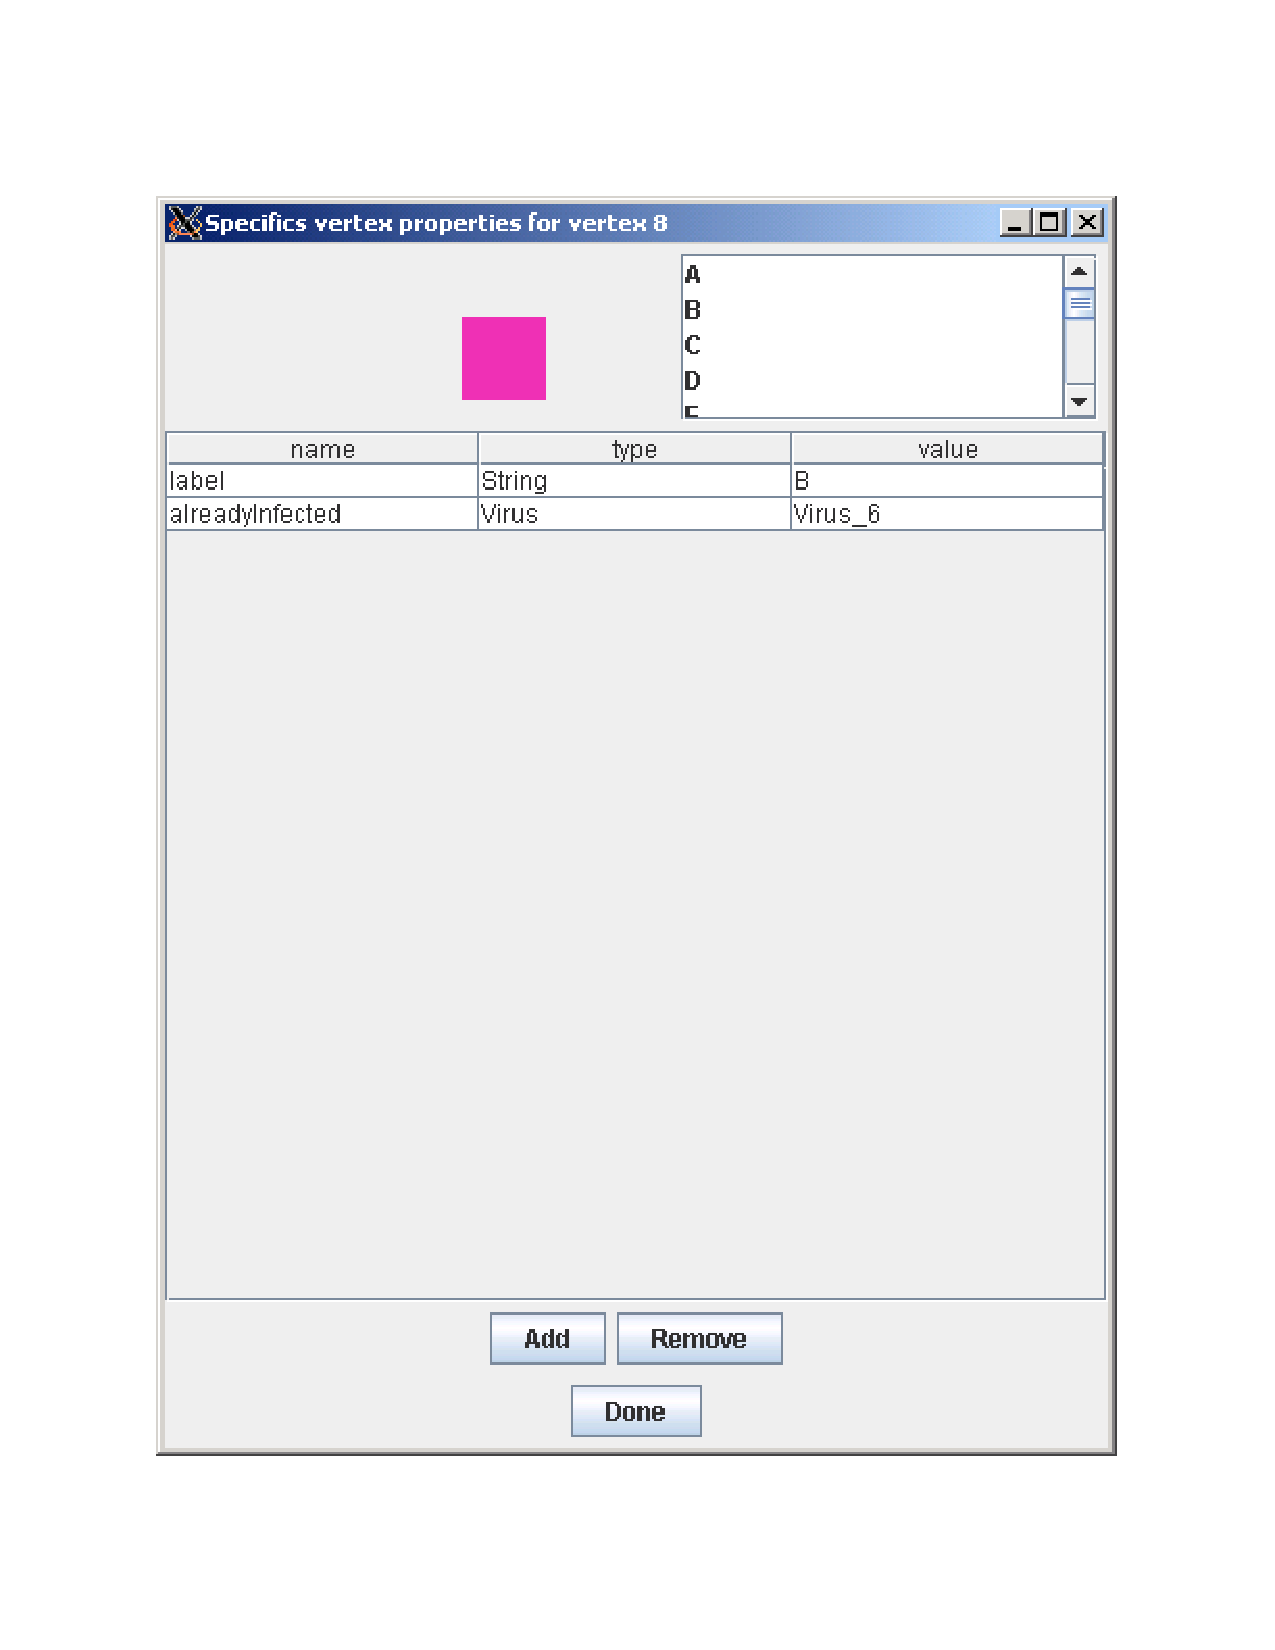
\includegraphics[width=10cm]{fonctionnement-vertex-properties}
  \caption{Visualtisation des informations du whiteboard d'un sommet}
  \label{fig:fonctionnement-vertex-properties}
\end{figure}

Lorsque tous les agents ont termin�s, la simulation se termine � son
tour et en informe l'utilisateur.

\begin{figure}[ht]
  \centering
  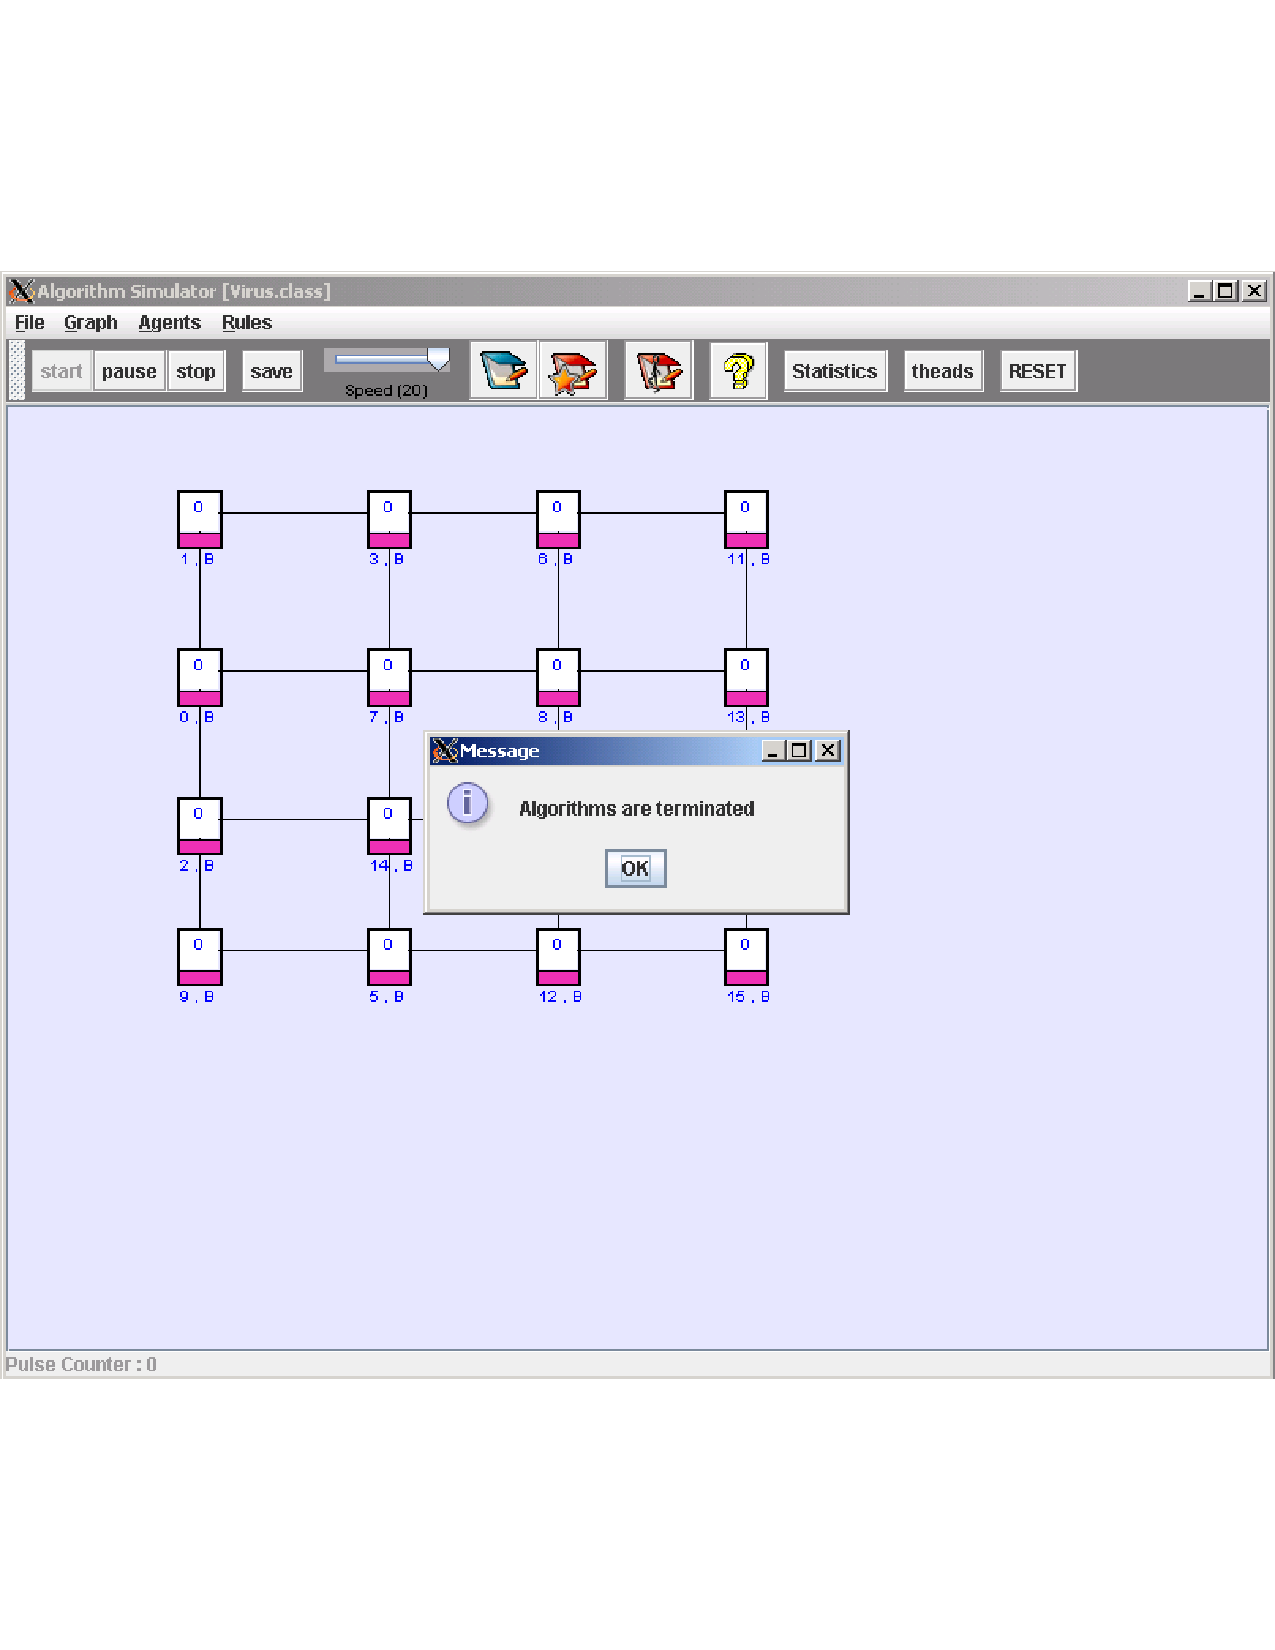
\includegraphics[width=10cm]{fonctionnement-simu-terminated}
  \caption{Les algorithmes sont termin�s, tous les agents sont mort}
  \label{fig:fonctionnement-simu-terminated}
\end{figure}

Des statistiques param�trables peuvent �galement etre �tablies. Pour
cela l'utilisateur doit avoir pr�alablement programm� sa classe de
calcul de statistiques et l'avoir compil� (voir le Manuel
d'utilisation).

\begin{figure}[ht]
  \centering
  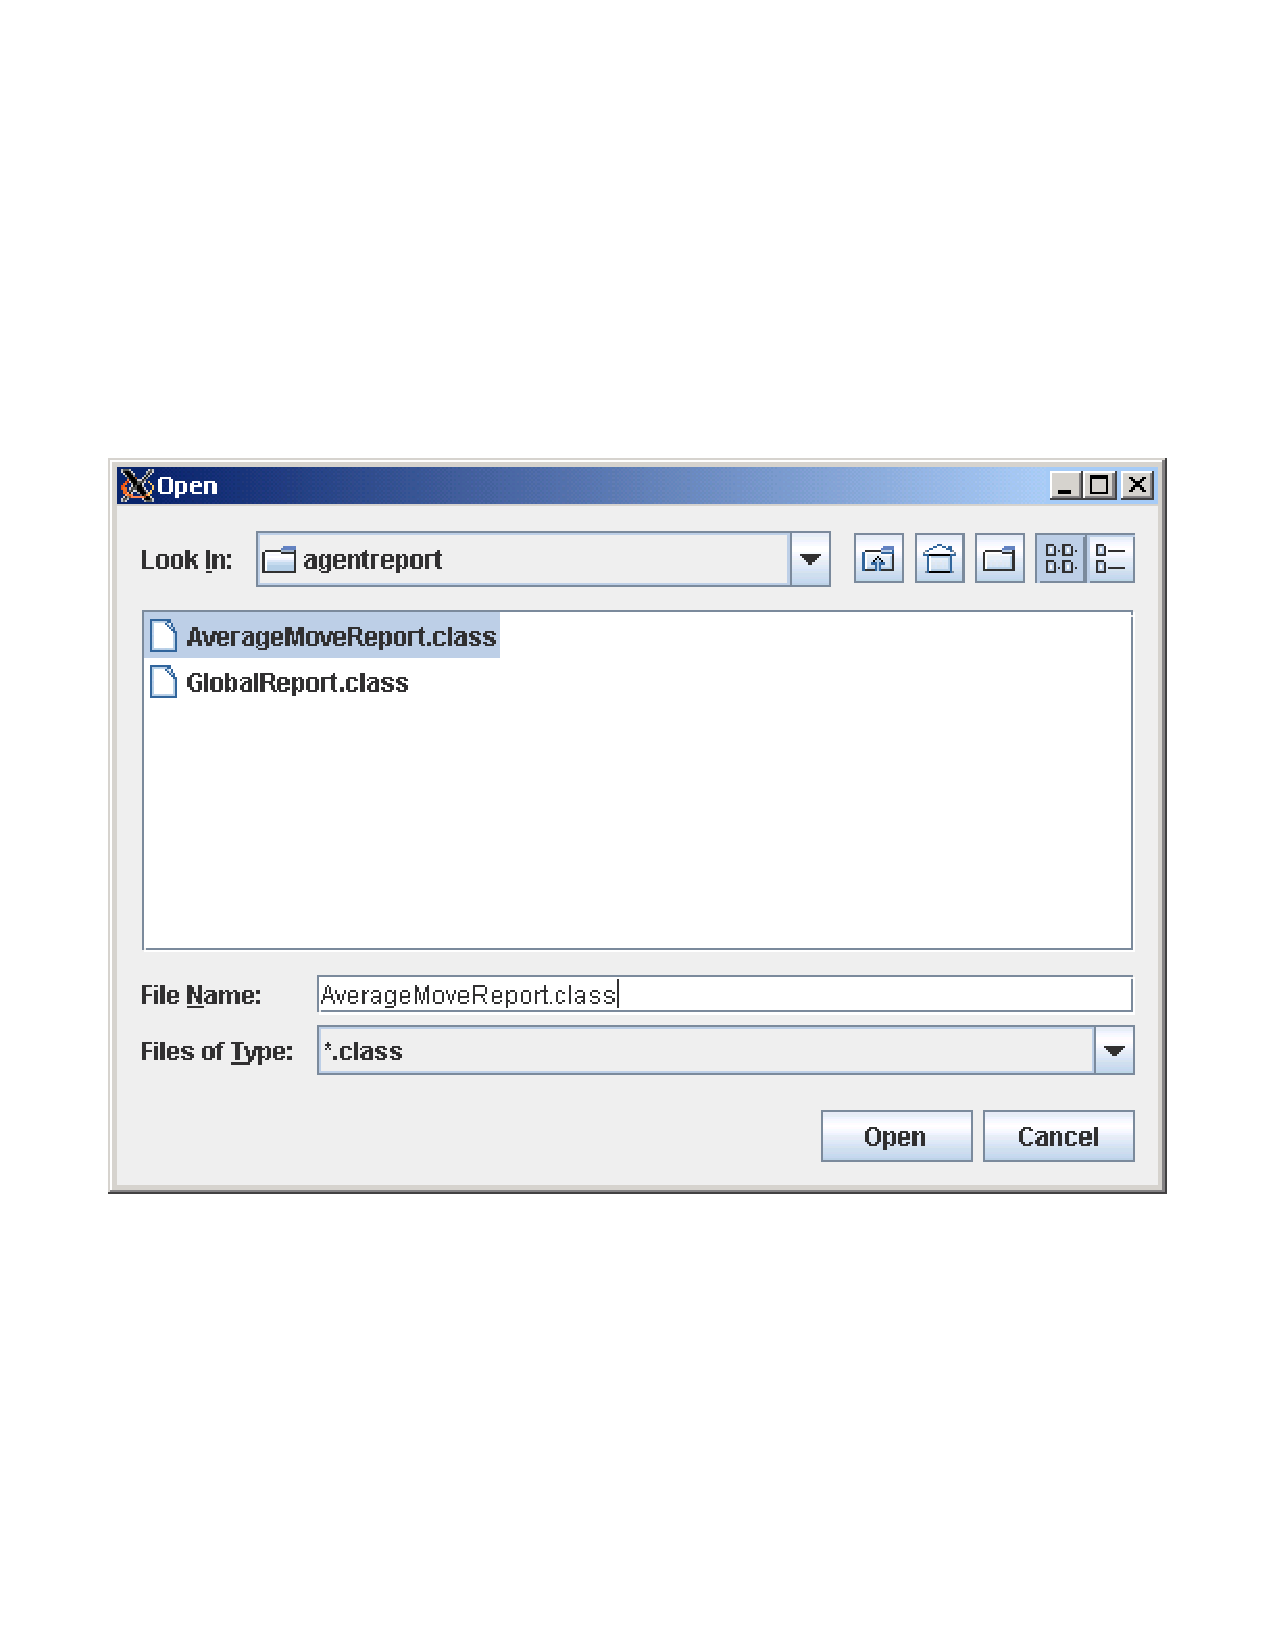
\includegraphics[width=10cm]{fonctionnement-choix-stats}
  \caption{Choix de la m�thode de calcul des satistiques}
  \label{fig:fonctionnement-choix-stats}
\end{figure}


\begin{figure}[ht]
  \centering
  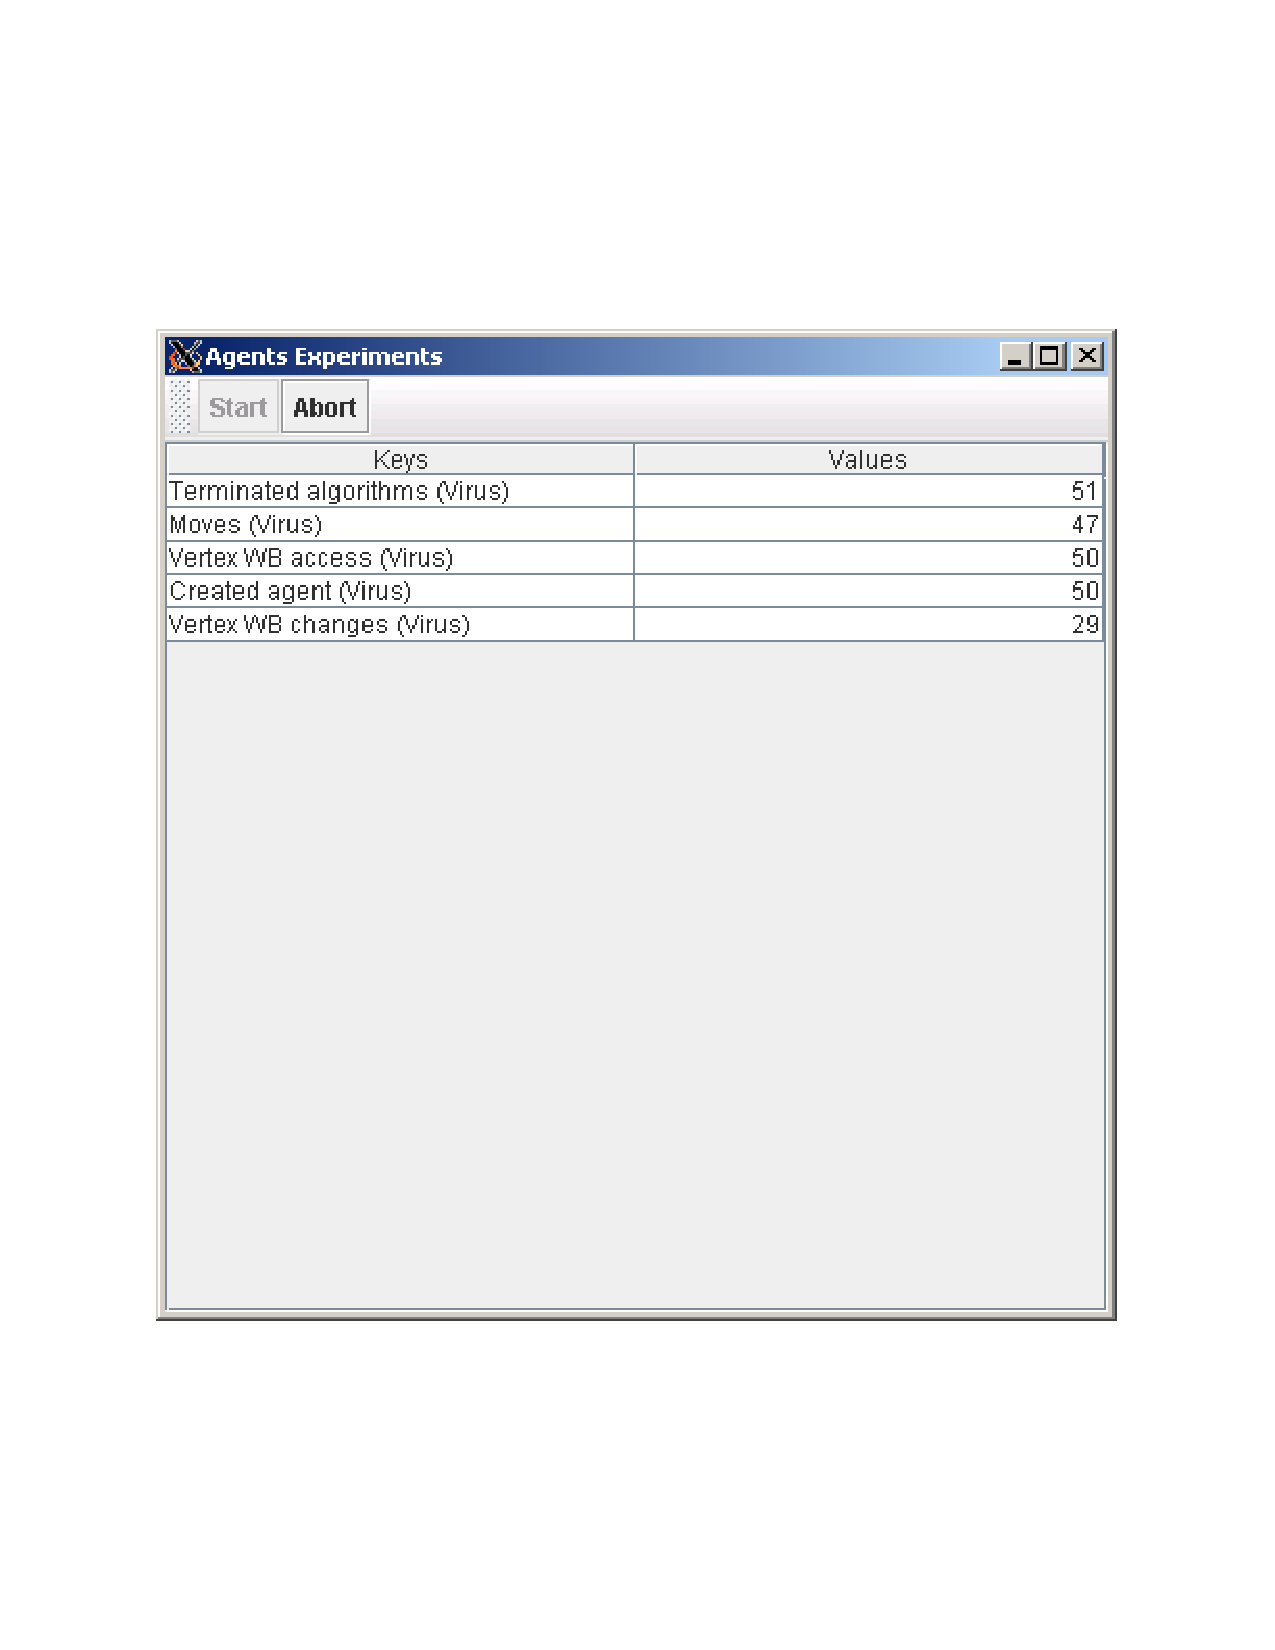
\includegraphics[width=10cm]{fonctionnement-stats}
  \caption{R�sultats du calcul de nos statistiques}
  \label{fig:}
\end{figure}



%\paragraph{Ecriture d'un algorithme}




%%% Local Variables: 
%%% mode: latex 
%%% TeX-master:  "rapport" 
%%% TeX-PDF-mode: t 
%%% coding:latin-1 
%%% End:

%screenshot
%comment on �crit un algo
%xavier
\chapter{Bilan}
%% Local Variables: 
%% mode: latex
%% TeX-master: t
%% TeX-PDF-mode: t
%% coding: latin-1
%% End:
%nada

\chapter{Lexique}

Vous  trouverez  ci-dessous les  d�finitions  relatives aux  principaux
termes et sigles utilis�s dans la r�alisation du cahier des charges.


\begin{description}

\item[Algorithmique distribu�e] : Cette partie de l'algorithmique
s'int�resse aux algorithmes s'ex�cutant sur plusieurs unit�s de calcul
en m�me temps. Le mod�le th�orique d'un r�seau dans ce cadre est un
graphe dont les sommets (ou noeuds) sont des machines ou processeurs
et les ar�tes des connexions.

\item[Agent   mobile]   :   Entit�   autonome   de   calcul   qui   se
d�place \cite{agentBook}.

\item[A.P.I.]   :  Application  Programming  Interface.   Ensemble  de
prototypes   de  fonctions   accessibles   depuis  l'ext�rieur   d'une
biblioth�que. C'est l'interface publique de la biblioth�que.

\item[Door  ou porte]  : une  porte est  une connexion  �  partir d'un
sommet du graphe  vers un autre sommet.  Les  portes sont num�rot�es �
partir de 0.

\item[ENSEIRB]   :    �cole   Nationale   Sup�rieure   d'�lectronique,
Informatique et Radiocommunications de Bordeaux \cite{enseirb}.

\item[Javadoc] :  outil qui  permet de g�n�rer  de la  documentation �
  partir du code source et des commentaires Java.

\item[LaBRI]  :  Laboratoire Bordelais  de  Recherche en  Informatique
\cite{labri}.

\item[PFA]  :  Projet  de  Fin  d'Ann�e. Module  de  programmation  de
  quatri�me semestre  de fili�re informatique �  l'ENSEIRB.  Ce module
  consiste en  l'�laboration d'un  projet sur une  dur�e de 3  mois en
  groupe de 7  � 8 personnes. Il a pour but  de nous familiariser avec
  les m�thodes  de travail  en groupe sur  des projets de  plus longue
  dur�e  et   de  plus  grande   taille  que  ceux  dont   nous  avons
  l'habitude. Dans le cadre du pr�sent projet, les chercheurs du LaBRI
  constituent donc les clients auxquels  on doit rendre des comptes en
  tant que prestataires.

\item[thread  ou processus  l�ger]  :  un thread  est  similaire �  un
  processus : il ex�cute  un ensemble d'instructions. Toutefois, l� ou
  chaque processus  poss�de sa  propre m�moire virtuelle,  les threads
  qui appartiennent au m�me processus p�re partagent un m�me partie de
  sa m�moire virtuelle.

\item[\visidia]   :  Visualization   and  Simulation   of  Distributed
Algorithms ou  Visualisation et Simulation  des Algorithmes Distribu�s
\cite{visidiaLaBRI}.

\end{description}



%% Local Variables:
%% mode: latex
%% coding: latin-1
%% TeX-master: "main"
%% End:
\chapter{Bibliographie}





%% Local Variables:
%% mode: latex
%% coding: latin-1
%% TeX-master: "main"
%% End:

\end{document}

%% Local Variables: 
%% mode: latex
%% TeX-master: t
%% TeX-PDF-mode: t
%% coding: latin-1
%% End:
